\section*{Contexte}\label{contexte}

\ifprof
\else
Les satellites d'observation terrestre sont une aide importante dans de nombreux domaines et en particulier pour tenter de prédire les
phénomènes liés à l'environnement ou les tremblements de terre. Dans ce contexte, DEMETER est un satellite français d'observation géophysique :
Detection of Electro Magnetic Emissions Transmitted from Earthquake Regions. Les objectifs scientifiques de DEMETER sont multiples :
\begin{itemize}
\item étudier les perturbations ionosphériques dues aux activités sismiques ;
\item étudier les perturbations ionosphériques dues aux activités humaines ;
\item étudier les conséquences pré- et post-sismiques dans l'ionosphère ;
\item apporter une contribution à la compréhension des mécanismes de génération de ces perturbations ;
\item donner une information globale sur l'environnement électromagnétique de la Terre à l'altitude du satellite.
\end{itemize}

\begin{figure}[!htb]
\begin{center}
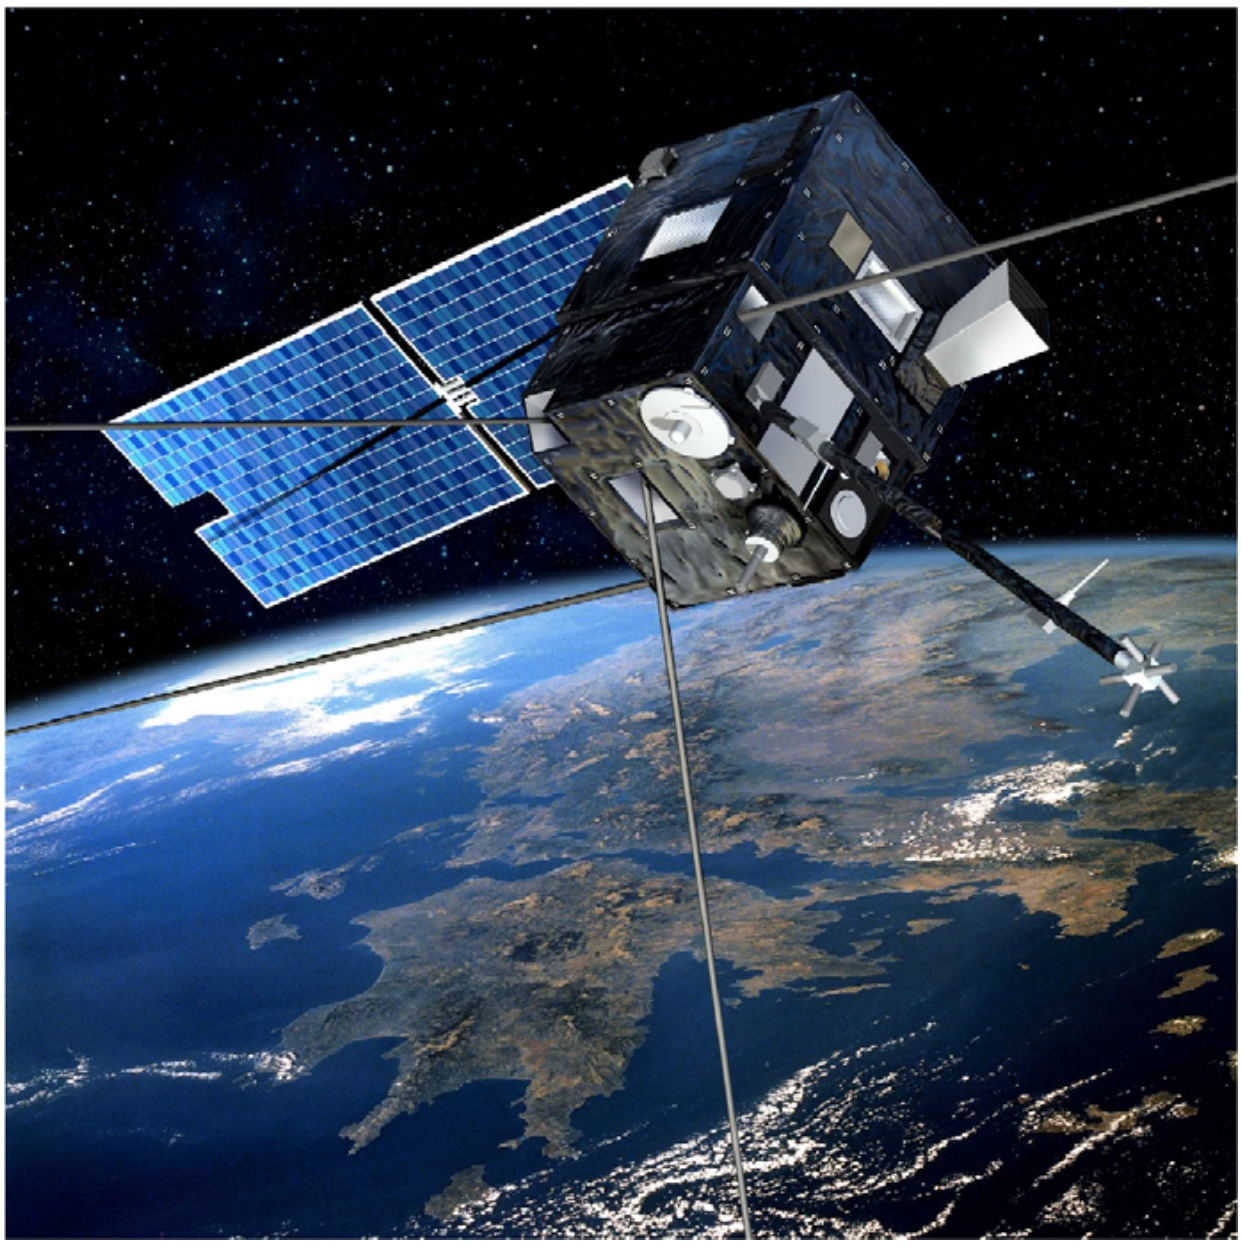
\includegraphics[width=0.5\textwidth]{images/images1.jpg}
\caption{Satellite d'observation géophysique DEMETER \label{fig1}}
\end{center}
\end{figure}



Ce sujet a pour objet la conception et la validation du système de contrôle d'attitude et d'orbite (ou SCAO), l'attitude désignant
l'orientation du satellite par rapport à un trièdre de référence. Le contrôle des satellites est souvent fondé autour de solutions
complémentaires :
\begin{itemize}
\item la propulsion par jet d'hydrazine ;  
\item les roues de réaction ;
\item les magnétocoupleurs.  
\end{itemize}

Cette étude s'intéresse plus particulièrement au pointage fin ou mode
nominal opérationnel (MNO) dont la finalité est d'assurer une précision
d'attitude de $0,04^{\circ}$. Dans ce mode, seuls les roues de réaction et les
magnéto-coupleurs sont utilisés.

L'étude se décompose en trois parties. La partie \ref{partieI} porte sur l'analyse
de la plateforme utilisée pour la mission DEMETER. Les objectifs de la
partie \ref{partieII} sont d'une part la mise en place des modèles dynamiques qui
seront exploités pour la définition de la loi de commande, d'autre part
la vérification du dimensionnement des actionneurs utilisés pour cette
mission. Enfin, dans la partie \ref{partieIII}, il s'agira d'une part de déterminer
et de valider les lois de commande pour le contrôle d'attitude du
satellite, d'autre part de proposer des solutions permettant d'assurer
que l'ensemble du système, en particulier les actionneurs, répond aux
exigences du cahier des charges.

%\FloatBarrier
\fi
\section{Étude préliminaire de la plateforme utilisée pour le satellite}\label{partieI}

\ifprof
\else
Un satellite est un engin spatial sans pilote dont l'architecture est
fortement caractérisée par la mission qu'il doit accomplir. Il est
constitué de deux sous-ensembles :

\begin{itemize}
\item la charge utile comprenant toute l'instrumentation scientifique
  embarquée spécifique à la mission ;
\item la plateforme comprenant la structure mécanique du satellite et tous
  les éléments assurant l'ensemble des fonctions nécessaires à
  l'utilisation de la charge utile (système de contrôle d'attitude et
  d'orbite ou SCAO, régulation de la puissance électrique, régulation
  thermique, communications avec la station au sol, ...).
\end{itemize}

Dans le cas du satellite DEMETER, ces deux sous-systèmes sont même
séparés physiquement, la plateforme étant fondée sur un modèle générique
appelé Myriade et destiné au développement de micro-satellites du même
type que DEMETER.

La structure de la plateforme Myriade, montrée dépliée sur la
\autoref{fig2}, est un parallélépipède de base carrée de 60
centimètres de côté, et de hauteur 50 centimètres. Elle est constituée :

\begin{itemize}
\item d'une plaque de base massive en aluminium assurant l'interface avec le
  lanceur et susceptible d'accueillir le module de propulsion ;
\item de quatre panneaux latéraux en nid d'abeilles permettant la fixation
  des équipements ;
\item d'un panneau supérieur, également en nid d'abeilles, destiné à
  recevoir la charge utile.
\end{itemize}

\begin{figure}[!htb]
\begin{center}
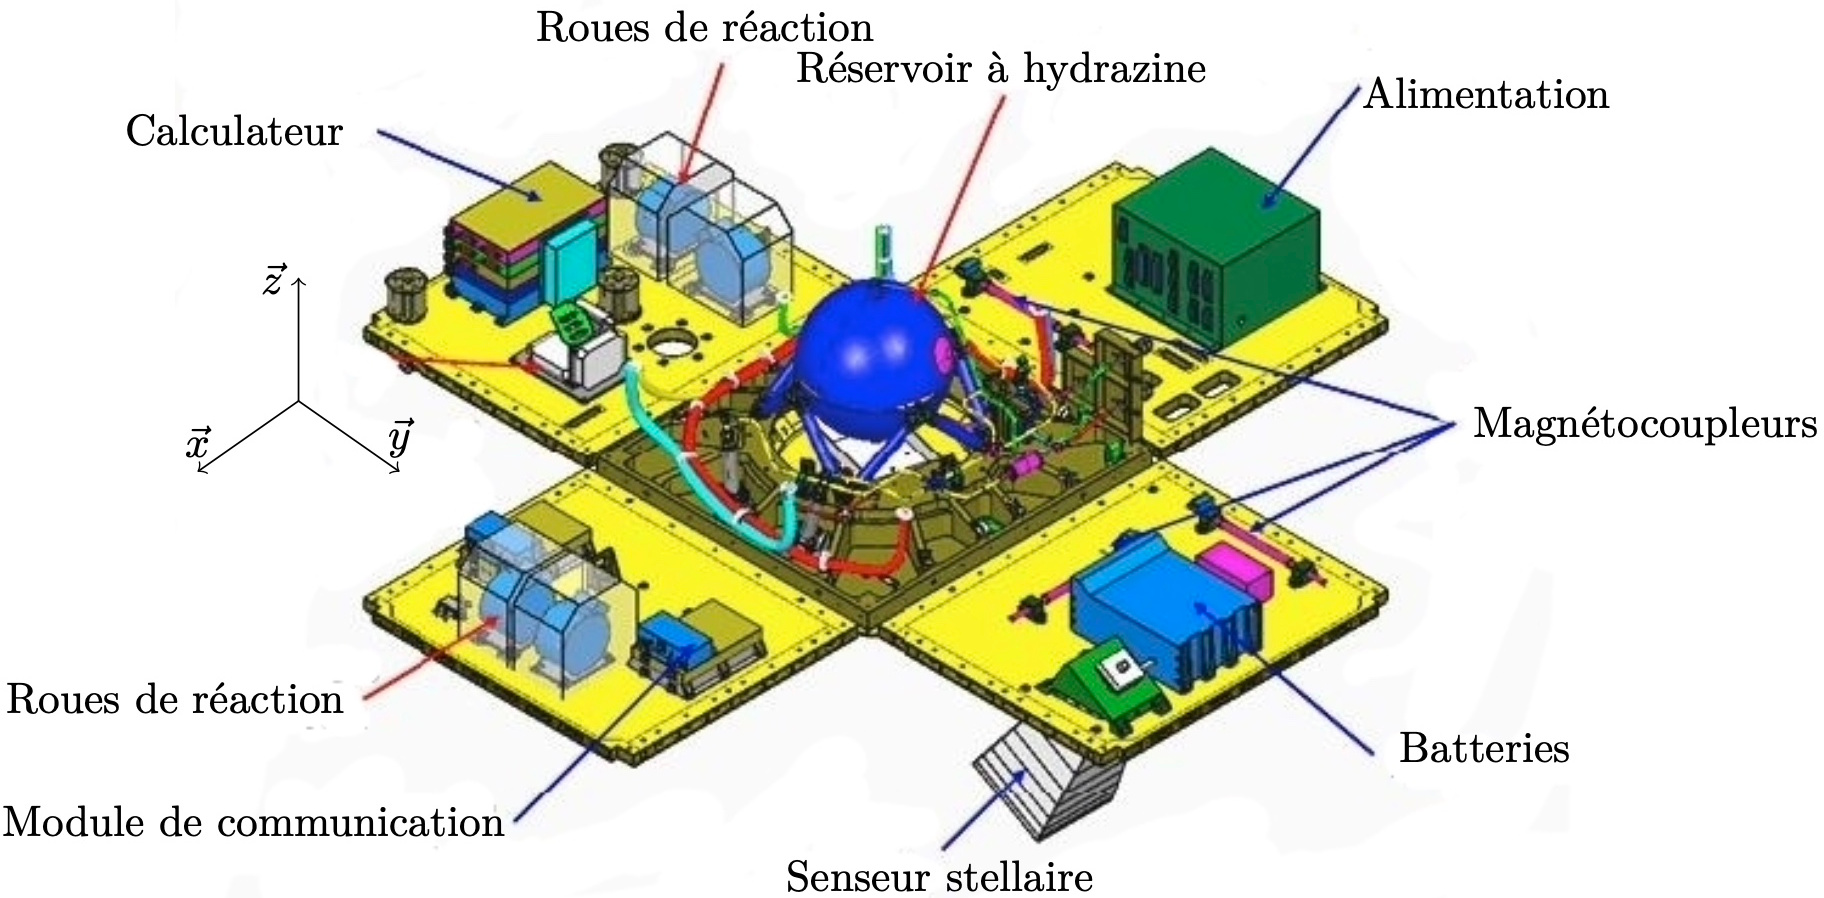
\includegraphics[width=0.48\textwidth]{images/images2.jpg}
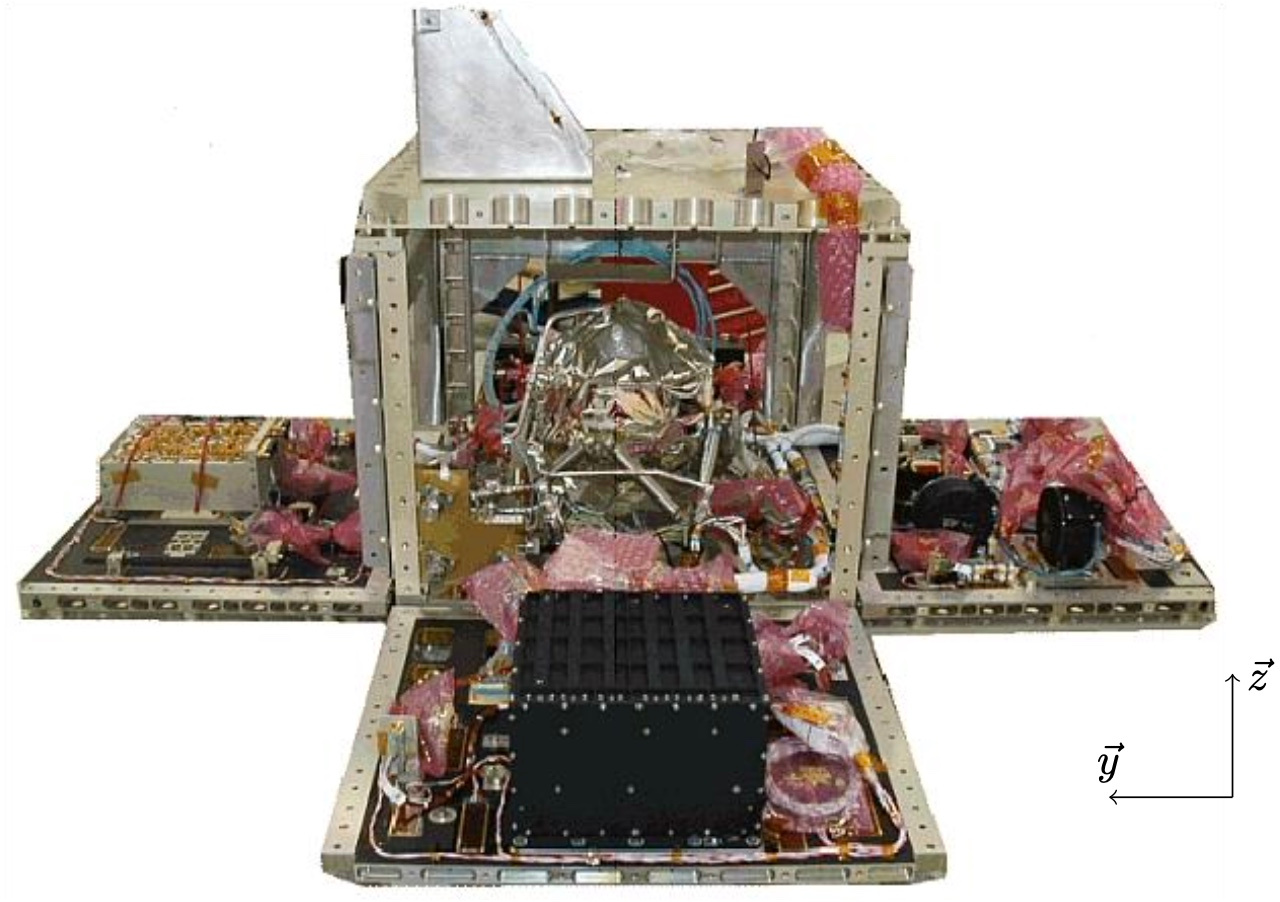
\includegraphics[width=0.48\textwidth]{images/images3.jpg}
\caption{Plateforme Myriade (panneaux latéraux dépliés) \label{fig2}}
\end{center}
\end{figure}

Les équipements sont les suivants :
\begin{itemize}
\item un module de propulsion utilisant quatre moteurs à hydrazine qui
  permet un contrôle de l'orbite du satellite ;
\item quatre roues de réaction et trois magnétocoupleurs qui assurent un
  contrôle de l'orientation du satellite ;
\item un senseur stellaire qui permet de mesurer l'orientation du satellite
  vis-à-vis des étoiles observées ;
\item un calculateur qui élabore les grandeurs de commande en fonction de
  l'écart entre les valeurs mesurées et les consignes imposées ;
\item des thermistances qui rendent possible un contrôle de la température ;
\item un module de communication avec la station au sol ;
\item un système de batteries alimentées par deux panneaux solaires
  articulés et orientables.
\end{itemize}

Le satellite DEMETER est placé sur une orbite polaire (c'est-à-dire une
orbite circulaire dont le plan contient les deux pôles terrestres) dans
le référentiel géocentrique qui est un référentiel galiléen, d'origine
le centre de la Terre O et de directions stellaires fixées. On le notera $R_g\quadruplet{O}{\vect{X_0}}{\vect{Y_0}}{\vect{Z_0}}$. L'altitude du satellite
est \emph{h} = \SI{710}{km}.

On fait l'hypothèse que le satellite n'est soumis qu'à l'action de la Terre modélisée par :
$$
\torseur{\T\left(\text{Terre}\to \text{Satellite}\right)}=\torseurLigne{G}{-\mathcal{G}\dfrac{Mm}{\left(R+h\right)^2}\vect{Z}}{\vect{0}}
$$


où $G$ est le centre d'inertie du satellite de masse $m = \SI{129}{kg}$, 
$M = \SI{5,97e24}{kg}$ 
et $R = \SI{6356}{km}$
sont respectivement la masse et le rayon de la Terre supposée sphérique.

$\vect{Z}$ désigne le vecteur unitaire colinéaire (de même sens) au vecteur reliant
le centre de la Terre au centre d'inertie du satellite et $\mathcal{G} =\SI{6,67e-11}{m^{3}  kg^{-1} s^{-2}}$ est la
constante universelle de la gravitation.

Ainsi on peut définir un référentiel orbital $R_o\quadruplet{G}{\vect{X}}{\vect{Y}}{\vect{Z}}$ qui se déduit du référentiel $R_g$ par une rotation autour de la direction $\vect{Y}_0=\vect{Y}$ d'angle $\alpha=\couple{\vect{Z}_0}{\vect{Z}}=\couple{\vect{X}_0}{\vect{X}}$.


 Ainsi,$$
\vect{OG}=\left(R+h\right)\vect{Z}
$$

Compte tenu de l'orbite choisie pour DEMETER, ses panneaux solaires ne
captent la lumière du Soleil que pendant une durée limitée à chaque
révolution. Le courant n'est généré par les cellules des panneaux que
pendant ces périodes éclairées qui permettent alors de recharger le
système de batteries. Les caractéristiques de gestion de l'énergie sur
DEMETER sont précisées sur le cahier des charges partiel du tableau \ref{tab3}.


\begin{table}[!htb]
\begin{center}
\begin{tabular}{|c|c|}
\hline
Durée d'éclairement des panneaux solaires (à chaque révolution) & 65 min\\ \hline
Capacité totale du système de batteries & $\SI{15}{A h}$\\ \hline
Nombre de circuits électriques à alimenter & 44\\ \hline
Intensité maximale dans chaque circuit & $\SI{0,6}{A}$\\ \hline
\end{tabular}
\caption{Cahier des charges partiel concernant la gestion de
l'énergie de DEMETER \label{tab3}}
\end{center}
\end{table}

\fi
  
%
%\question{\label{q_1}}\textit{Calculer la résultante dynamique du satellite dans son mouvement par rapport au référentiel géocentrique $R_g$ (noté $\vect{R_d}(\text{satellite}/R_g))$. \label{q1}}
%\question{\label{q_2}}\textit{Applique le théorème de la résultante dynamique au satellite par rapport au référentiel géocentrique et obtenir deux équations différentielles en fonction de $\alpha(t)$.}
%\question{\label{q_3}}\textit{Calculer la vitesse linéaire du centre d'inertie du satellite par
%  rapport au référentiel géocentrique $\Vert\vect{V}(G/R_g)\Vert$ et le taux de rotation orbital $\dot{\alpha}$ en fonction de $\mathcal{G}$, $M$, $m$, $R$ et $h$.}
%\question{\label{q_4}}\textit{En déduire la pulsation orbitale
%$\omega_0=2\pi/T$ et la période de révolution du satellite autour de la Terre $T$.}
%\question{\label{q_5}}\textit{Calculer la durée pendant laquelle, sur une période de révolution, le
%  satellite est masqué par la Terre et n'est donc pas éclairé par la
%  lumière du Soleil. Vérifier si la capacité du système de batteries est
%  suffisante pour faire face à la consommation du satellite pendant ces
%  intervalles d'obscurité.}
  
  

\question{\label{q_3}}\textit{Calculer la vitesse linéaire du centre d'inertie du satellite par
  rapport au référentiel géocentrique. En déduire la pulsation orbitale
$\omega_0=2\pi/T$, où $T$ est la période de révolution du satellite autour de la Terre .}
\ifprof
\begin{corrige}
Rrésultante dynamique du satellite dans son mouvement par rapport au référentiel géocentrique $R_g$ :
$\vect{R_d}(\text{satellite}/R_g)=m\cdot \vect{a}(G\in \text{satellite}/R_0)=\dfrac{\dd^2\vect{OG}}{\dd t^2\vert_{R_g}} =\dfrac{\dd^2(R+h)\vect{Z}}{\dd t^2\vert_{R_g}}$.

Or par la formule de dérivation vectorielle
$ \dfrac{\dd\vect{Z}}{\dd t\vert_{R_g}}=\dot{\alpha}\vect{X}$ 
et $\dfrac{\dd\vect{X}}{\dd t\vert_{R_g}}=-\dot{\alpha}\vect{Z}$.

Ainsi on obtient,
$
\boxed{
\vect{R_d}(\text{satellite}/R_g)=m\cdot (R+h)\left(\ddot{\alpha}\vect{X}-\dot{\alpha}^2\vect{Z}\right)
}$.

Application du théorème de la résultante dynamique au satellite.
\begin{itemize}
\item \textbf{Bilan des actions mécaniques :}
Le satellite est uniquement soumis à l'attraction gravitationnelle de la terre : 
$
\torseur{\T\left(\text{Terre}\to \text{satellite}\right)}=\torseurl{-\mathcal{G}\dfrac{Mm}{\left(R+h\right)^2}\vect{Z}}{\vect{0}}{G}$.
\item Le théorème de la résultante dynamique appliqué au satellite d'écrit : 
$\vect{R_d}(\text{satellite}/R_g)=\vect{R}(\text{Terre} \to \text{satellite})$

On en déduit deux équations : 
$
\begin{array}{c}
\cdot \vect{X}\\
\cdot \vect{Z}\\
\end{array}
\quad 
\left\{
\begin{array}{c}
m\cdot (R+h)\ddot{\alpha}=0\\
-m\cdot (R+h)\dot{\alpha}^2=-\mathcal{G}\dfrac{Mm}{\left(R+h\right)^2}\\
\end{array}
\right.
$.
\end{itemize}


De plus, $\Vert\vect{V}(G/R_g)\Vert=\Vert\dfrac{\dd\vect{OG}}{\dd t\vert_{R_g}}\Vert
=\Vert\dfrac{\dd (R+h)\vect{Z}}{\dd t\vert_{R_g}}\Vert=(R+h)\dot{\alpha}
$.

Avec la deuxième équation du TRD, on a : $(R+h)\dot{\alpha}=\sqrt{\mathcal{G}\dfrac{M}{\left(R+h\right)}}$.


On en déduit :  $ \boxed{\dot{\alpha}=\sqrt{\mathcal{G}\dfrac{M}{\left(R+h\right)^3}}}$
et 
$\boxed{ \Vert\vect{V}(G/R_g)\Vert=\sqrt{\mathcal{G}\dfrac{M}{\left(R+h\right)}}}$.


On en déduit en faisant l'application numérique : 
$\omega_0=\dot{\alpha}=\dfrac{\mathcal{G}M}{\left(h+R\right)^3}\approx\SI{1,06e-3}{rad.s^{-1}}$.


On obtient alors comme période de révolution :  $T=\dfrac{2\pi}{\omega_0}=\SI{5914}{s}$.

Ainsi T correspond à 1h38min et 34 s

\end{corrige}
\else
\fi

\question{\label{q_5}}\textit{Calculer la durée pendant laquelle, sur une période de révolution, le
  satellite est masqué par la Terre et n'est donc pas éclairé par la
  lumière du Soleil. Vérifier si la capacité du système de batteries est
  suffisante pour faire face à la consommation du satellite pendant ces
  intervalles d'obscurité.}
\ifprof
\begin{corrige}
Soit $T_{\text{mas}}$  la durée pendant laquelle, sur une période de révolution, le
  satellite est masqué par la Terre et n'est donc pas éclairé par la
  lumière du Soleil.
  
  $  T_{\text{mas}}=T-T_{\text{éclairement}}=\SI{33}{min}\SI{34}{s}=\SI{2014}{s}$
  \
  On peut calculer la durée de consommation de la batterie par  : 
  $  t_{\text{conso}}=\dfrac{44\times 0,6}{15}=\SI{1,76}{h}>\SI{33}{min}\SI{34}{s}=\SI{2014}{s}$
  
  Le cahier des charges est bien respecté.
\end{corrige}
\else
\fi


\section{Modélisation dynamique du système satellite}\label{partieII}

\begin{obj}
L'objet de cette partie est la définition et la mise en place de modèles
dynamiques du satellite et des actionneurs. Les modèles établis seront
utilisés pour l'étude de la loi de commande en vue d'asservir l'attitude
du satellite, c'est-à-dire son orientation par rapport à des directions
de référence.
\end{obj}

\ifprof
\else
La phase de modélisation s'articule en deux étapes. Dans la première, il
s'agit d'une part d'établir le modèle dynamique du satellite dans son
environnement en l'assimilant à un solide indéformable, d'autre part de
mettre en évidence les couples perturbateurs. Dans une deuxième étape,
la modélisation des actionneurs à roue de réaction est effectuée et leur
dimensionnement vérifié.
\fi

\subsection{Modèle de satellite rigide}
\ifprof
\else
On s'intéresse ici à l'évolution de l'orientation du satellite quand il
n'est soumis qu'à l'action de la Terre. Pour cela, on introduit les
référentiels suivants :

\begin{itemize}
\item $R_g\quadruplet{O}{\vect{X_0}}{\vect{Y_0}}{\vect{Z_0}}$ référentiel géocentrique, supposé galiléen, d'origine le centre de la Terre (supposée parfaitement sphérique) ;
\item $R_o\quadruplet{O}{\vect{X}}{\vect{Y}}{\vect{Z}}$ référentiel orbital, d'origine le centre d'inertie du satellite, où $\vect{X}$ est le vecteur unitaire tangent à l'orbite circulaire du satellite autour de la Terre, $\vect{Z}$ est le vecteur unitaire colinéaire à $\vect{OG}$ et de même sens et $\vect{Y}$ complète le repère orthonormé direct ainsi obtenu ;
\item $R_s\quadruplet{G}{\vect{x}}{\vect{y}}{\vect{z}}$ référentiel du satellite, d'origine le centre d'inertie du satellite, et où $\couple{G}{\vect{x}}$, $\couple{G}{\vect{y}}$ et $\couple{G}{\vect{z}}$ sont les axes principaux d'inertie du satellite.
\end{itemize}

Le référentiel orbital est en rotation uniforme autour de l'axe $\couple{O}{\vect{Y}}$ par
rapport au référentiel géocentrique, de telle sorte que le vecteur
vitesse de rotation instantanée associé s'écrit $\vect{\Omega}(R_o/R_g)=\omega_0\cdot \vect{Y}$ où $\omega_0$ est la pulsation
orbitale (constante) définie dans la partie précédente.

Le passage du référentiel orbital au référentiel du satellite se fait
par l'intermédiaire des trois angles de Cardan définis sur la
\textbf{Figure \ref{fig4}} :

\begin{figure}[!htb]
\begin{minipage}[c]{0.3\textwidth}
\begin{itemize}
\item $\phi$ est l'angle de roulis ;
\item $\theta$ est l'angle de tangage ;
\item $\psi$ est l'angle de lacet.
\end{itemize}
\end{minipage}
\begin{minipage}[c]{0.7\textwidth}
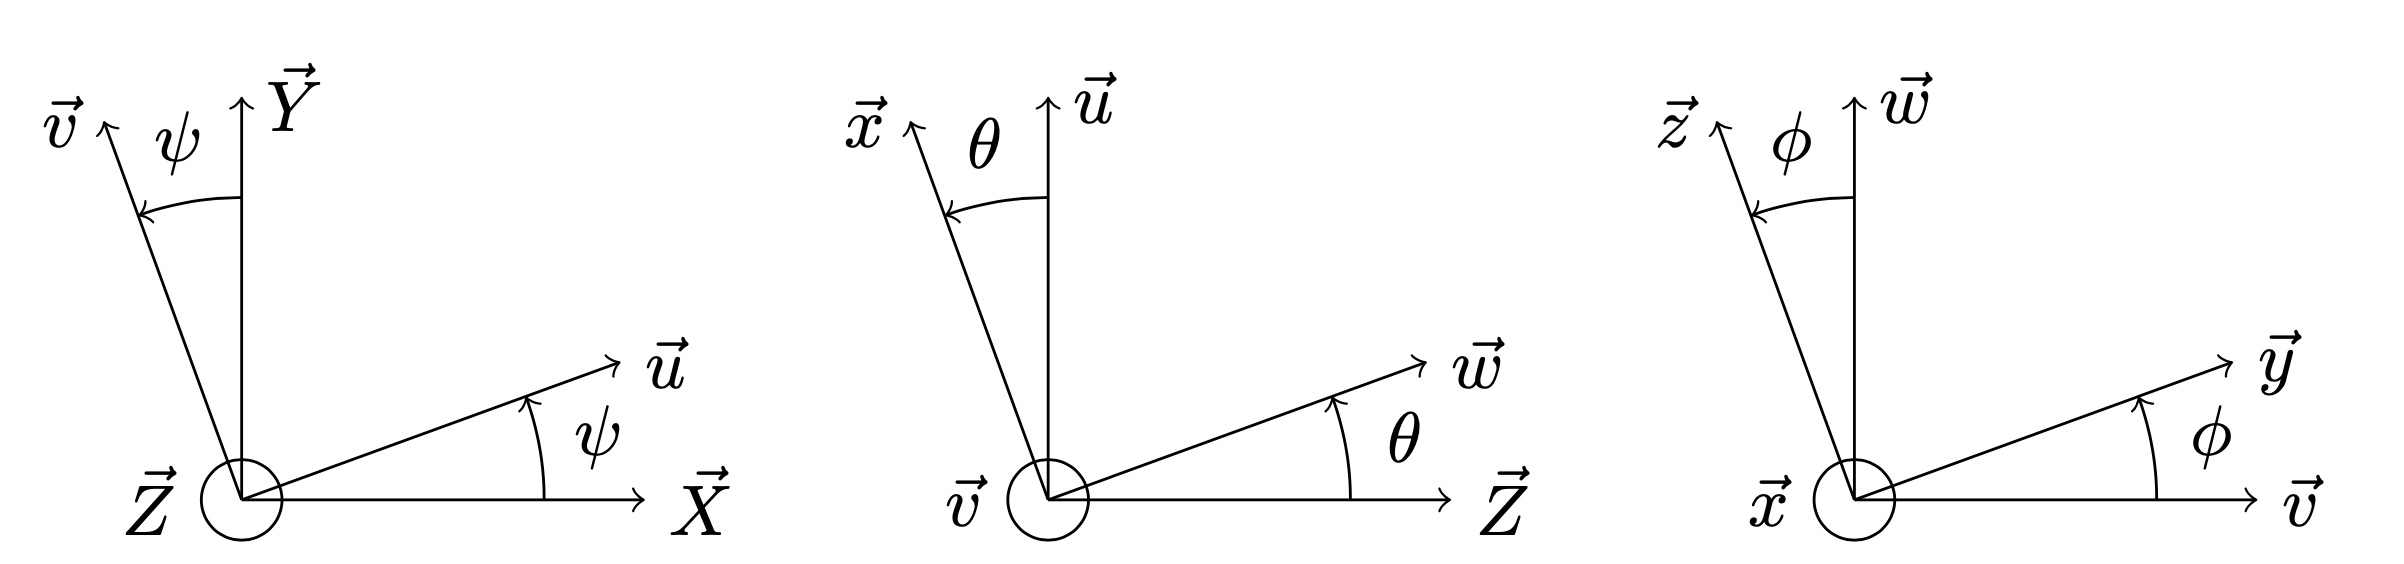
\includegraphics[width=0.95\textwidth]{images/image4.jpg}
\end{minipage}
\caption{ Définition des angles de lacet, tangage et roulis. \label{fig4}}
\end{figure}

\fi

\question{\label{q_6}}\textit{Calculer les composantes du vecteur $\vect{Z}$ dans la base \triplet{\vect{x}}{\vect{y}}{\vect{z}} liée au satellite. Pour quelles valeurs des angles de roulis, tangage et lacet a-t-on un << pointage Terre >>, c'est-à-dire $\vect{Z}=\vect{z}$ ?}
\ifprof
\begin{corrige}
$\vect{Z}=\cos\theta\left(\cos\phi\vect{z}+\sin\phi\vect{y}\right)-\sin\theta\vect{x}$ .
De plus $\vect{Z}=\vect{z}\Leftrightarrow \theta=\phi=k\cdot \pi \text{avec k } \in \mathbb{N}$.

On a un pointage de la terre si $\theta=\phi=0$ ou si $\theta=\phi=\pi$, il n'y a pas de contrainte sur $\psi$.
\end{corrige}
\else
\fi

\ifprof
\else
On suppose que le satellite est en mode de pointage fin (tel qu'il sera
étudié dans la partie \ref{partieIII}) : les angles de roulis, tangage et
lacet sont donc très petits :
$$
\begin{array}{ccc}
\phi=o(1) &  \theta=o(1) & \psi=o(1)
\end{array}
$$

De même, on suppose que les dérivées temporelles de ces angles sont très
petites devant la pulsation orbitale :

$$
\begin{array}{ccc}
\dot{\phi}=o(\omega_0) & \dot{\theta}=o(\omega_0) & \dot{\psi}=o(\omega_0)
\end{array}
$$

On obtient alors l'expression suivante (admise), à l'ordre un en $\left(\phi,\theta;\psi;\dot{\phi};\dot{\theta};\dot{\psi}\right)$, pour
le vecteur vitesse de rotation instantanée $\vect{\Omega}(R_s/R_g)$ du référentiel du satellite
par rapport au référentiel géocentrique :

$$
\vect{\Omega}(R_s/R_g)=\left(\psi\omega_0+\dot{\phi}\right)\vect{x}+\left(\omega_0+\dot{\theta}\right)\vect{y}+\left(-\phi\omega_0+\dot{\psi}\right)\vect{z}.
$$

On considère en outre que le satellite est un solide indéformable
unique, de caractéristiques suivantes :

\begin{itemize}
\item  centre d'inertie $G$ tel que $\Vert \vect{OG} \Vert= \SI{7066}{km}$ ;
\item masse $m = \SI{129}{kg}$ ;
\item matrice d'inertie :
$$
I(G,s)=
\left(
\begin{array}{ccc}
I_x & 0 & 0 \\ 
0 & I_y & 0 \\ 
0 & 0 & I_z
\end{array}
\right)_{\triplet{\vect{x}}{\vect{y}}{\vect{z}}} 
$$
 avec $I_{x}= \SI{31,4}{kg m^2}$, $I_{y} = \SI{35,7}{kg.m^2}$, $I_{z} = \SI{21,2}{kg.m^2}$.
\end{itemize}

Il est soumis, en plus de l'action de la Terre, supposée uniforme, à des
actions mécaniques supplémentaires :

$$
\torseur{\T\left(\text{extérieur}\to \text{satellite}\right)}=\torseurLigne{G}{R_x^{\text{ext}}\vect{x}+R_y^{\text{ext}}\vect{y}+R_z^{\text{ext}}\vect{z}}{C_x^{\text{ext}}\vect{x}+C_y^{\text{ext}}\vect{y}+C_z^{\text{ext}}\vect{z}}.
$$

\fi


\question{\label{q_7}}\textit{Exprimer littéralement, au point G et dans le repère \triplet{\vect{x}}{\vect{y}}{\vect{z}}, le moment dynamique $\vect{\delta}(G,R_s/R_g$ à l'ordre un en $\left(\dot{\phi};\dot{\theta};\dot{\psi},\ddot{\phi};\ddot{\theta};\ddot{\psi}\right)$ du mouvement du satellite par rapport au référentiel géocentrique.}
\ifprof
\begin{corrige}

A l'ordre 1, on a : $
\vect{\Omega}(R_s/R_g)=\left(\psi\omega_0+\dot{\phi}\right)\vect{x}+\left(\omega_0+\dot{\theta}\right)\vect{y}+\left(-\phi\omega_0+\dot{\psi}\right)\vect{z}
$.

Comme le moment dynamique est exprimé en $G$ (centre d'inertie du satellite) on obtient l'équation suivante : 
$
\vDelta[G]{R_s}{R_g}=\left[\frac{\dd \vSigma[G]{R_s}{R_g}}{\dd t}\right]_{R_g}
$.


Or, $\vSigma[G]{R_s}{R_g}=\overline{\overline{I}}_G(S)\cdot \vect{\Omega}(R_s/R_g)$.

$$
\vSigma[G]{R_s}{R_g}=\left(
\begin{array}{ccc}
I_x & 0 & 0 \\ 
0 & I_y & 0 \\ 
0 & 0 & Iz
\end{array}
\right)_{\triplet{\vect{x}}{\vect{y}}{\vect{z}}} 
\cdot 
\left(
\begin{array}{c}
\psi\omega_0+\dot{\phi} \\ 
\omega_0+\dot{\theta} \\ 
-\phi\omega_0+\dot{\psi}
\end{array}
\right)_{\triplet{\vect{x}}{\vect{y}}{\vect{z}}} 
=
\left(
\begin{array}{c}
I_x\left(\psi\omega_0+\dot{\phi} \right)\\ 
I_y\left(\omega_0+\dot{\theta} \right)\\ 
I_z\left(-\phi\omega_0+\dot{\psi}\right)
\end{array}
\right)_{\triplet{\vect{x}}{\vect{y}}{\vect{z}}} .
$$

Ainsi on déduit en appliquant la formule de dérivation vectorielle : $
\vDelta[G]{R_s}{R_g}=\left[\frac{\dd \vSigma[G]{R_s}{R_g}}{\dd t}\right]_{R_g}+\vect{\Omega}(R_s/R_g)\wedge  \vSigma[G]{R_s}{R_g}$. 

Ainsi,
$$
\vDelta[G]{R_s}{R_g}=\left(
\begin{array}{c}
I_x\left(\dot{\psi}\omega_0+\ddot{\phi} \right)\\ 
I_y\ddot{\theta}\\ 
I_z\left(-\dot{\phi}\omega_0+\ddot{\psi}\right)
\end{array}
\right)_{\triplet{\vect{x}}{\vect{y}}{\vect{z}}} 
+
\left(
\begin{array}{c}
\psi\omega_0+\dot{\phi} \\ 
\omega_0+\dot{\theta} \\ 
-\phi\omega_0+\dot{\psi}
\end{array}
\right)_{\triplet{\vect{x}}{\vect{y}}{\vect{z}}} 
\wedge
\left(
\begin{array}{c}
I_x\left(\psi\omega_0+\dot{\phi} \right)\\ 
I_y\left(\omega_0+\dot{\theta} \right)\\ 
I_z\left(-\phi\omega_0+\dot{\psi}\right)
\end{array}
\right)_{\triplet{\vect{x}}{\vect{y}}{\vect{z}}}.
$$

Soit,
$$
\vDelta[G]{R_s}{R_g}=\left(
\begin{array}{c}
I_x\left(\dot{\psi}\omega_0+\ddot{\phi} \right)+I_z\left(-\phi\omega_0+\dot{\psi}\right)\left(\omega_0+\dot{\theta}\right)-I_y\left(\omega_0+\dot{\theta} \right)\left(-\phi\omega_0+\dot{\psi}\right)
\\ 
I_y\ddot{\theta}+I_x\left(\psi\omega_0+\dot{\phi} \right)\left(-\phi\omega_0+\dot{\psi}\right)-I_z\left(-\phi\omega_0+\dot{\psi}\right)\left(\psi\omega_0+\dot{\phi} \right)\\ 
I_z\left(-\dot{\phi}\omega_0+\ddot{\psi}\right)
+I_y\left(\omega_0+\dot{\theta} \right)\left(\psi\omega_0+\dot{\phi} \right)
-I_x\left(\psi\omega_0+\dot{\phi} \right)\left(\omega_0+\dot{\theta} \right)
\end{array}
\right)_{\triplet{\vect{x}}{\vect{y}}{\vect{z}}}.$$

En linéarisant au 1\up{er} ordre, donc en considérant les termes du second ordre nuls on obtient la solution suivante :
$$
\vDelta[G]{R_s}{R_g}=\left(
\begin{array}{c}
I_x\left(\dot{\psi}\omega_0+\ddot{\phi} \right)+\left(I_z-I_y\right)\left(\omega_0\dot{\psi}-\omega_0^2\phi\right)
\\ 
I_y\ddot{\theta}\\ 
I_z\left(-\dot{\phi}\omega_0+\ddot{\psi}\right)
+\left(I_y-I_x \right)\left(\omega_0\dot{\phi}+\omega_0^2\psi\right)
\end{array}
\right)_{\triplet{\vect{x}}{\vect{y}}{\vect{z}}}.
$$

\end{corrige}
\else
\fi

\question{\label{q_8}\label{q_05}}\textit{En déduire les trois équations scalaires du mouvement faisant
  intervenir les angles de roulis, tangage et lacet \triplet{\phi}{\theta}{\psi} ainsi que leurs dérivées temporelles $\left(\dot{\phi};\dot{\theta};\dot{\psi},\ddot{\phi};\ddot{\theta};\ddot{\psi}\right)$.}
\ifprof
\begin{corrige}
L'application du principe fondamental de la dynamique au satellite et au
point $G$ (centre d'inertie) et plus particulièrement le théorème du
moment dynamique associé conduit à l'équation suivante~:
$\vDelta[G]{R_s}{R_g}=\vect{M}_G(\text{ext}\to s)$.

 En l'occurrence, il y en a que deux actions mécaniques extérieures :
\begin{itemize}
\item action de la Terre sur le satellite de moment nul en $G$; 
\item actions mécaniques extérieures supplémentaires de moment en G~: $ C_x^{\text{ext}}\vect{x}+C_y^{\text{ext}}\vect{y}+C_z^{\text{ext}}\vect{z}$.
\end{itemize}

Ainsi dans la base $R_s$ nous avons les 3 équations supplémentaires~:

$$
\begin{array}{c}
\cdot \vect{x}\\
\cdot \vect{y}\\
\cdot \vect{z}\\
\end{array}
\left\{
\begin{array}{c}
I_x\left(\dot{\psi}\omega_0+\ddot{\phi} \right)+\left(I_z-I_y\right)\left(\omega_0\dot{\psi}-\omega_0^2\phi\right)=C_x^{\text{ext}}\\
I_y\ddot{\theta}=C_y^{\text{ext}}\\
I_z\left(-\dot{\phi}\omega_0+\ddot{\psi}\right)
+\left(I_y-I_x \right)\left(\omega_0\dot{\phi}+\omega_0^2\psi\right)=C_z^{\text{ext}}\\
\end{array}
\right.
$$

\end{corrige}
\else
\fi


On note $\Phi(p)$, $\Psi(p)$, $C_x^{\text{ext}}(p)$ et $C_z^{\text{ext}}(p)$ les transformées de Laplace de $\phi(t)$, $\psi(t)$, $C_z^{\text{ext}}(t)$ et $C_y^{\text{ext}}(t)$ respectivement. 
%
\question{\label{q_9}}\textit{Montrer, en prenant des conditions initiales nulles, que l'on peut écrire :}
$$
H_{\Phi x}(p)=\dfrac{\Phi(p)}{C_x^{\text{ext}}(p)}=\dfrac{\kappa_2+\beta p^2}{\left(\kappa_1+\alpha p^2\right)\left(\kappa_2+\beta p^2\right)+\gamma^2p^2}\\
\\
H_{\Phi z}(p)=\dfrac{\Phi(p)}{C_z^{\text{ext}}(p)}=\dfrac{\gamma p}{\left(\kappa_1+\alpha p^2\right)\left(\kappa_2+\beta p^2\right)+\gamma^2p^2}\\
$$
\textit{ où l'on précisera les expressions de $\kappa_1$, $\kappa_2$, $\alpha$, $\beta$ et $\gamma$ en fonction de $I_x$, $I_y$, $I_z$ et $\omega_0$.}

\ifprof
\begin{corrige}

Les équations de la question précédente conduisent au système suivant~:
$$
\left\{
\begin{array}{c}
I_x\ddot{\phi} +\left(I_y-I_z\right)\omega_0^2\phi=C_x^{\text{ext}}+\left(I_y-I_z-I_x\right)\dot{\psi}\omega_0\\
I_z\ddot{\psi} +\left(I_y-I_x\right)\omega_0^2\psi=C_z^{\text{ext}}+\left(I_x-I_y+I_z\right)\dot{\phi}\omega_0\\
\end{array}
\right.
$$

En passant dans le domaine de Laplace avec les conditions initiales nulles, nous obtenons le système suivant~:
$$
\left\{
\begin{array}{c}
\left[I_x p^2+ \left(I_y-I_z\right)\omega_0^2\right]\Phi(p)=C_x^{\text{ext}}(p)+\left(I_y-I_z-I_x\right)p \omega_0\Psi(p)\\
\left[I_z p^2 +\left(I_y-I_x\right)\omega_0^2\right]\Psi(p)=C_z^{\text{ext}}(p)+\left(I_x-I_y+I_z\right)p\omega_0 \Phi(p)\\
\end{array}
\right.
$$

On peut mettre la 1\textsuperscript{ère} et la 3\textsuperscript{ème} équation sous la forme du système suivant.
$$ \lambda_1\cdot \Phi(p)=C_x^{\text{ext}}(p)+\lambda_2\Psi(p) \quad \quad \text{(1)} $$
$$ \mu_1 \cdot \Psi(p)=C_z^{\text{ext}}(p)+\mu_2(p) \Phi(p) \quad \quad \text{(2)} $$

Pour avoir $H_{\Phi z}(p)=\dfrac{\Phi(p)}{C_z^{\text{ext}}(p)}$ on peut appliquer le principe de superposition en
considérant $C_x^{\text{ext}}(p)=0$. 

Puis dans un second temps il est proposé d'étudier $H_{\Phi x}(p)=\dfrac{\Phi(p)}{C_x^{\text{ext}}(p)}$ en
considérant $C_z^{\text{ext}}(p)=0$.

\begin{itemize}
\item 1\textsuperscript{er} cas~  $C_x^{\text{ext}}(p)=0$ : 
  \begin{itemize}
  \item (1) devient $\lambda_1\cdot \Phi(p)=\lambda_2\Psi(p)$
  \item (2) devient alors~: $\left(\mu_1 \dfrac{\lambda_1}{\lambda_2}-\mu_2\right) \cdot \Phi(p)=C_z^{\text{ext}}(p)$
  \item Ainsi on en déduit~: $
H_{\Phi z}(p)=\dfrac{\Phi(p)}{C_z^{\text{ext}}(p)}=\dfrac{\lambda_2}{\mu_1\cdot \lambda_1-\mu_2\cdot \lambda_2}
$.
 Ainsi : 
$$
H_{\Phi z}(p)=\dfrac{\left(I_y-I_z-I_x\right)p\omega_0}{\left[I_z p^2 +\left(I_y-I_x\right)\omega_0^2\right]\left[I_x p^2+ \left(I_y-I_z\right)\omega_0^2\right]-\left(I_x-I_y+I_z\right)p\omega_0\left(I_y-I_z-I_x\right)p \omega_0}
$$
$$
=\dfrac{\left(I_y-I_z-I_x\right)p\omega_0}{I_xI_zp^4+\omega_0^2 p^2\left[I_z\cdot \left(I_y-I_z\right)+I_x\left(I_y-I_x\right)+\left(I_x-I_y+I_z\right)^2\right]+\left(I_y-I_x\right)\left(I_y-I_z\right)\omega_0^4}
$$
  
    \item Le résultat doit être de la forme suivante~:$
H_{\Phi z}(p)=\dfrac{\gamma p}{\left(\kappa_1+\alpha p^2\right)\left(\kappa_2+\beta p^2\right)+\gamma^2p^2}
$.
  
  \end{itemize}
\item 2\textsuperscript{ème} cas~:  $C_z^{\text{ext}}(p)=0$
  \begin{itemize}
  \item (2) devient $\mu_1\cdot \Phi(p)=\mu_2\cdot \psi(p)$
  \item  (2) devient alors~: $\left(\lambda_1\cdot \dfrac{\mu_1}{\mu_2}-\lambda_2\right)\Phi(p)=C_x^{\text{ext}}(p)$
  \item Ainsi on en déduit~: $
H_{\Phi x}(p)=\dfrac{\Phi(p)}{C_x^{\text{ext}}(p)}=\dfrac{\mu_2}{\lambda_1\cdot \mu_1-\lambda_2\cdot \mu_2}
$

$$
H_{\Phi x}(p)=\dfrac{I_z\cdot p^2+\left(I_y-I_x\right)\omega_0^2}{I_xI_zp^4+\omega_0^2 p^2\left[I_z\cdot \left(I_y-I_z\right)+I_x\left(I_y-I_x\right)+\left(I_x-I_y+I_z\right)^2\right]+\left(I_y-I_x\right)\left(I_y-I_z\right)\omega_0^4}
$$
  
  \item Le résultat doit être de la forme suivante~:
  $$
H_{\Phi x}(p)=\dfrac{\Phi(p)}{C_x^{\text{ext}}(p)}=\dfrac{\kappa_2+\beta p^2}{\left(\kappa_1+\alpha p^2\right)\left(\kappa_2+\beta p^2\right)+\gamma^2p^2}$$

$$
H_{\Phi z}(p)=\dfrac{\Phi(p)}{C_z^{\text{ext}}(p)}=\dfrac{\gamma p}{\left(\kappa_1+\alpha p^2\right)\left(\kappa_2+\beta p^2\right)+\gamma^2p^2}\\
$$
  

 \end{itemize}  
  
  \end{itemize}
  

\end{corrige}
\else
\fi

 

Tous calculs faits, il est possible de factoriser les dénominateurs de ces deux fonctions de transfert sous la forme suivante (admise) :
  
$$
\left(\kappa_1+\alpha p^2\right)\left(\kappa_2+\beta p^2\right)+\gamma^2p^2
=\left(\omega_0^2+p^2\right)\left[\left(I_y-I_z\right)\left(I_y-I_x\right)\omega_0^2+I_xI_z p^2\right]
$$
  
\question{\label{q_10}}\textit{Étudier la stabilité des modèles correspondant aux fonctions de transfert $H_{\Phi x}(p)$ et $H_{\Phi z}(p)$.}
\ifprof
\begin{corrige}
On admet la factorisation suivante du dénominateur

\begin{align*}
\left(k_1+\alpha\cdot p^2\right)\left(k_2+\beta\cdot p^2\right)+\gamma^2\cdot p^2=\left[I_xI_z\cdot p^2+\left(I_y-I_z\right)\left(I_y-I_x\right)\omega_0^2\right]\left(\omega_0^2+p^2\right)
\end{align*}
%
%On admet la factorisation suivante du dénominateur~:
%
Les 4 racines associées sont alors~: 
$$
j\omega_0
\quad
-j\omega_0
\quad
j\omega_0\sqrt{\dfrac{\left(I_y-I_z\right)\left(I_y-I_x\right)}{I_xI_y}}
\quad
-j\omega_0\sqrt{\dfrac{\left(I_y-I_z\right)\left(I_y-I_x\right)}{I_xI_y}}
$$


Car $I_y>I_x$ et $I_y>I_z$ car dans le cas de l'étude.

On peut remarquer qu'il s'agit de racines imaginaires purs donc le
système est quasi instable (ou juste stable). Pour une entrée bornée, la
sortie l'est également car le système est oscillant en l'absence de
perturbations extérieures.

En revanche, la sortie ne converge pas vers une valeur constante.

\end{corrige}
\else
\fi


\ifprof
\else
En réalité, l'action de la Terre n'est pas rigoureusement la même en
tout point du satellite. Un moment lié à ce <<~gradient de pesanteur~>> 
s'exerce donc sur le satellite.

On rappelle que l'action de la Terre exercée sur un petit volume
élémentaire de masse d\emph{m} situé au voisinage d'un point \emph{P} du
satellite s'écrit :
$$
\torseur{\T\left(\text{Terre}\to \dd m\right)}=\torseurLigne{P}{-\mathcal{G}\dfrac{M \dd m}{\Vert\vect{OP\Vert}^3}\vect{OP}}{\vect{0}}.
$$



où $O$ et $M = \SI{6e24}{kg}$ et $R = \SI{6356}{km}$
sont respectivement la masse et le rayon de la Terre et $\mathcal{G} =\SI{6,67e-11}{m^{3}.kg^{-1}.s^{-2}}$ est la
constante universelle de la gravitation. La \textbf{Figure \ref{fig5}} précise le paramétrage associé.


\begin{figure}[!htb]
\begin{center}
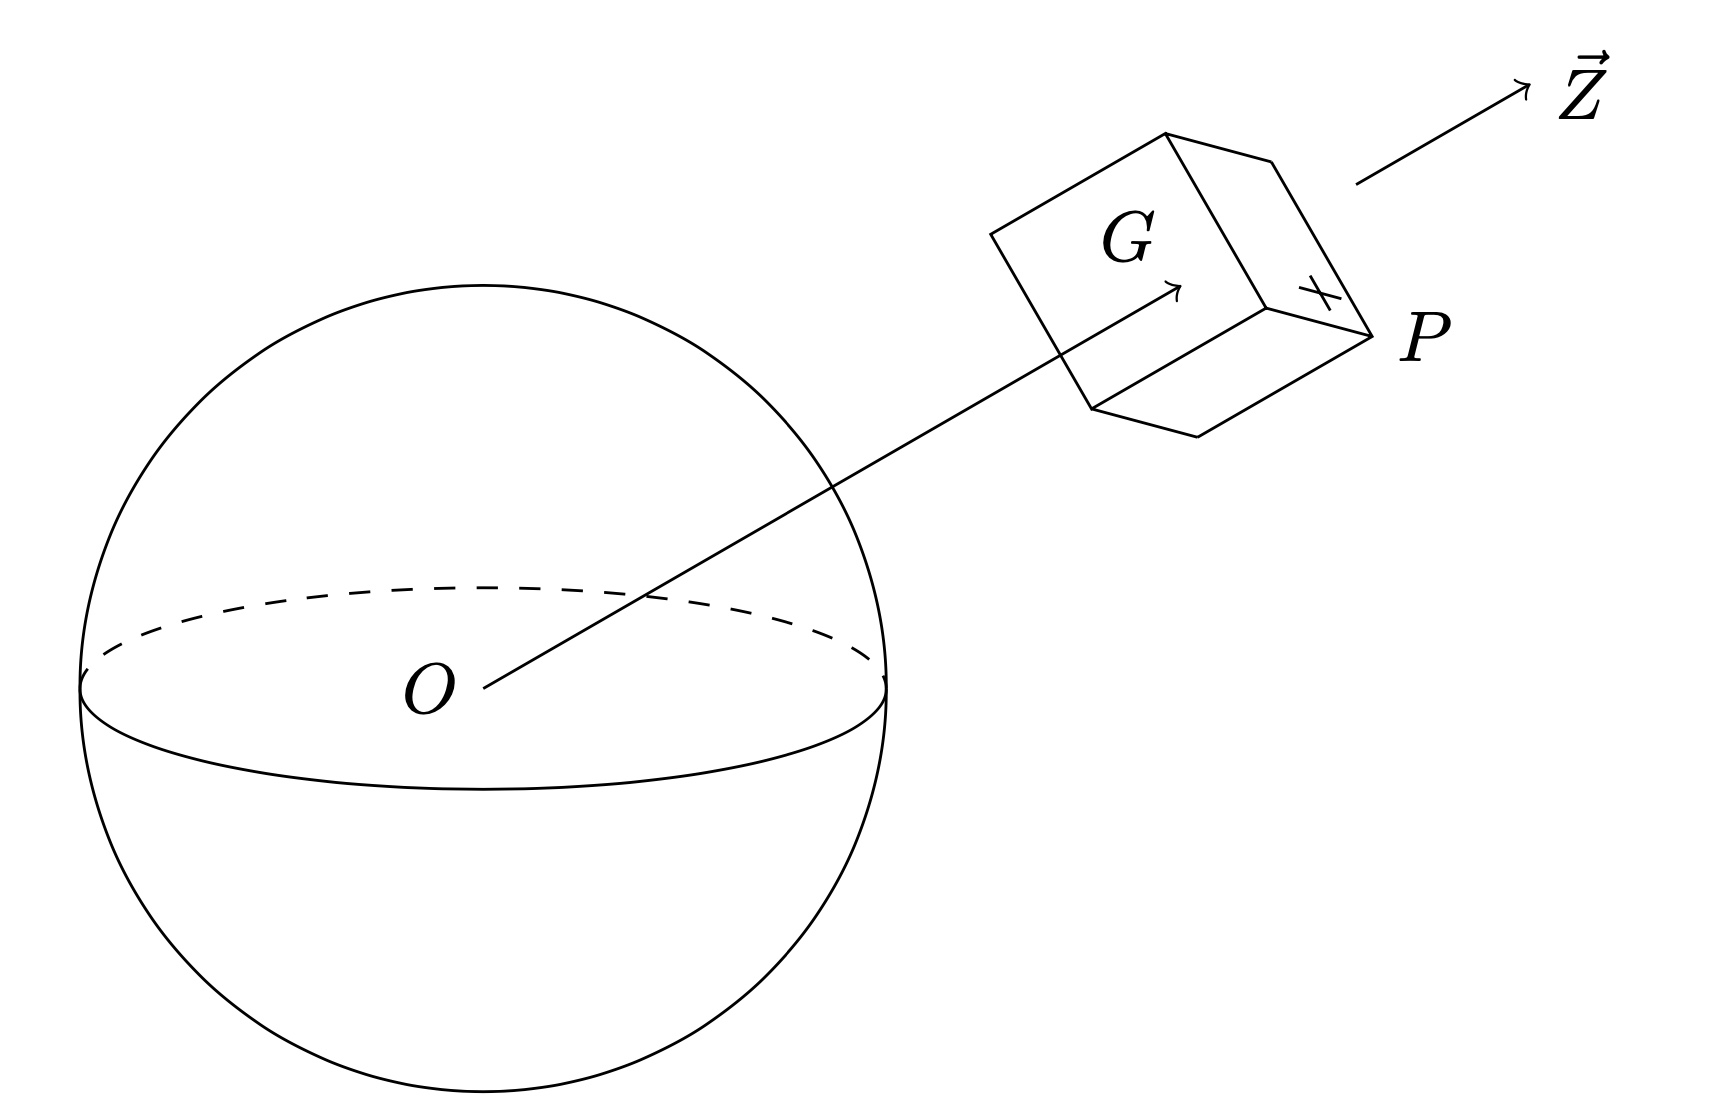
\includegraphics[width=0.5\textwidth]{images/images5.jpg}
\end{center}
\caption{Paramétrage pour la prise en compte du << gradient de pesanteur >> \label{fig5}}
\end{figure}

\fi

\question{\label{q_11}}\textit{ Montrer que le moment de l'action de la Terre sur le volume V du
  satellite peut s'exprimer en G par :}
$$
\vect{M}_G(\text{Terre}\to \text{satellite})=-\mathcal{G}\dfrac{M}{\Vert\vect{OP\Vert^3}}\int\int\int_V\left(\Vert\vect{OG}\Vert-3\vect{GP}\cdot\vect{Z}\right)\vect{GP}\wedge\vect{Z}\dd m
$$  
  
On utilisera pour cela sans démonstration le développement limité suivant :
  $$
  \Vert\vect{Z}+\varepsilon \vect{d} \Vert^n=1+n\varepsilon \vect{Z}\cdot \vect{a}+o(\varepsilon)
  $$
  où $\vect{a}$ est un vecteur arbitraire, $n$ un entier relatif quelconque et $\varepsilon$ un
  scalaire petit devant 1.
\ifprof
\begin{corrige}

\end{corrige}
\else
\fi


\ifprof
\else
On admet que le résultat de la \textbf{question précédente} donne pour
l'expression à l'ordre un en \triplet{\phi}{\theta}{\psi} du moment associé au «~gradient de
pesanteur ~ » :

$$
\vect{M}_G(\text{Terre}\to \text{satellite})=3\omega_0^2\left(I_z-I_y\right)\phi\vect{x}-3\omega_0^2\left(I_x-I_z\right)\theta\vect{z}
$$  

\fi


  
  
  \question{\label{q_12}}\textit{Déduire des trois équations scalaires obtenues précédemment du mouvement faisant
  intervenir les angles de roulis, tangage et lacet \triplet{\phi}{\theta}{\psi} ainsi que leurs dérivées temporelles $\left(\dot{\phi};\dot{\theta};\dot{\psi},\ddot{\phi};\ddot{\theta};\ddot{\psi}\right)$ les équations vérifiées
  par les angles de roulis, tangage et lacet dans le cas de la prise en
  compte du « gradient de pesanteur ». Étudier la stabilité du modèle
  correspondant à la fonction de transfert :}
    $$
  H_{\theta y}(p)=\dfrac{\Theta(p)}{C_y^{\text{ext}}(p)}
  $$
\textit{  où $\Theta(p)$ et $C_y^{\text{ext}}(p)$ sont les transformées de Laplace de $\theta(t)$ et $C_y^{\text{ext}}(t)$ respectivement. En
  supposant que l'étude de stabilité faite précédemment est encore
  valable ici, conclure à propos du choix de la géométrie du satellite.}
  \ifprof
\begin{corrige}

On rappelle les équations de la question  pour laquelle les
actions~mécaniques de pesanteur avaient un moment nul sous la forme
suivante:

$$
\begin{array}{c}
\cdot \vect{x}\\
\cdot \vect{y}\\
\cdot \vect{z}\\
\end{array}
\left\{
\begin{array}{c}
I_x\left(\dot{\psi}\omega_0+\ddot{\phi} \right)+\left(I_z-I_y\right)\left(\omega_0\dot{\psi}-\omega_0^2\phi\right)=C_x^{\text{ext}}\\
I_y\ddot{\theta}=C_y^{\text{ext}}\\
I_z\left(-\dot{\phi}\omega_0+\ddot{\psi}\right)
+\left(I_y-I_x \right)\left(\omega_0\dot{\phi}+\omega_0^2\psi\right)=C_z^{\text{ext}}\\
\end{array}
\right.
$$

A ces équations, on rajoute au PFD effectué précédemment  le moment précédemment calculé sous la forme suivante~:

$$
\begin{array}{c}
\cdot \vect{x}\\
\cdot \vect{y}\\
\cdot \vect{z}\\
\end{array}
\left\{
\begin{array}{c}
I_x\left(\dot{\psi}\omega_0+\ddot{\phi} \right)+\left(I_z-I_y\right)\left(\omega_0\dot{\psi}-\omega_0^2\phi\right)=C_x^{\text{ext}}+3\omega_0^2\left(I_z-I_y\right)\phi\\\
I_y\ddot{\theta}=C_y^{ext}-3\omega_0^2\left(I_x-I_z\right)\theta\\\
I_z\left(-\dot{\phi}\omega_0+\ddot{\psi}\right)
+\left(I_y-I_x \right)\left(\omega_0\dot{\phi}+\omega_0^2\psi\right)=C_z^{\text{ext}}\\
\end{array}
\right.
$$


On traduit l'équation selon $\vect{y}$ dans le domine de Laplace, en considérant
les CI nulles~: 
$$
I_y\cdot \Theta(p)\cdot p^2+3\omega_0^2\left(I_x-I_z\right)\Theta(p)=C_y^{\text{ext}}(p)
.$$

Ainsi on en déduit l'équation suivante~:
$ H_{\theta y}(p)=\dfrac{\Theta(p)}{C_y^{\text{ext}}(p)}=\dfrac{1}{I_y\cdot p^2+3\omega_0^2\left(I_x-I_z\right)}$.



$H_{\theta y}(p)$ est une fonction du 2\textsuperscript{nd} ordre qui peut être mise sous
la forme canonique suivante~: 
$$
  H_{\theta y}(p)=\dfrac{1}{3\omega_0^2\left(I_x-I_z\right)}\dfrac{1}{1+\dfrac{I_y}{3\omega_0^2\left(I_x-I_z\right)}\cdot p^2}.$$

On peut remarquer qu'il n'y a pas d'amortissement pour ce
2\textsuperscript{nd} ordre.

Les choix de géométrie effectués ($I_y>I_x>Iz$) permettent d'avoir 2 racines
complexes conjuguées à partie réelle nulle.

D'après l'étude de stabilité faite précédemment, on remarque que le
système est quasi instable (ou juste stable). Pour une entrée bornée, la
sortie l'est également car le système est oscillant en l'absence de
perturbations extérieures.

En revanche, la sortie ne converge pas vers une valeur constante.

NB~: Si l'on souhaite que le système devienne stable, il est nécessaire
d'introduire de l'amortissement (oscillations amorties convergentes vers
une valeur constante)


\end{corrige}
\else
\fi

 



\subsection{Actionneurs utilisés pour le contrôle d'attitude}

\ifprof
\else
La partie précédente a permis de mettre en évidence que l'orientation du
satellite avait tendance à évoluer naturellement tout au long de son
orbite si aucun dispositif de contrôle n'était prévu. Au moment
perturbateur créé par le phénomène de « gradient de pesanteur » vient
notamment s'ajouter un moment parasite supplémentaire, non étudié ici,
associé aux effets de traînée aérodynamique qui ne sont pas négligeables
à l'altitude où le satellite est en orbite et qui sont périodiques de
pulsation $2\omega_0$. Il est donc nécessaire d'utiliser des actionneurs pour agir
sur cette orientation de façon à assurer un pointage particulier.

Les actionneurs ont donc pour but de produire les couples nécessaires
pour compenser les moments perturbateurs décrits précédemment : il
s'agit de roues de réaction qui sont des roues de forte inertie axiale
dont on fait varier au cours du temps la vitesse de rotation autour de
leur axe de rotation. La \textbf{Figure \ref{fig6}} présente une photographie
d'une roue de réaction analogue à celles utilisées sur DEMETER.


\begin{figure}[!htb]
\begin{center}
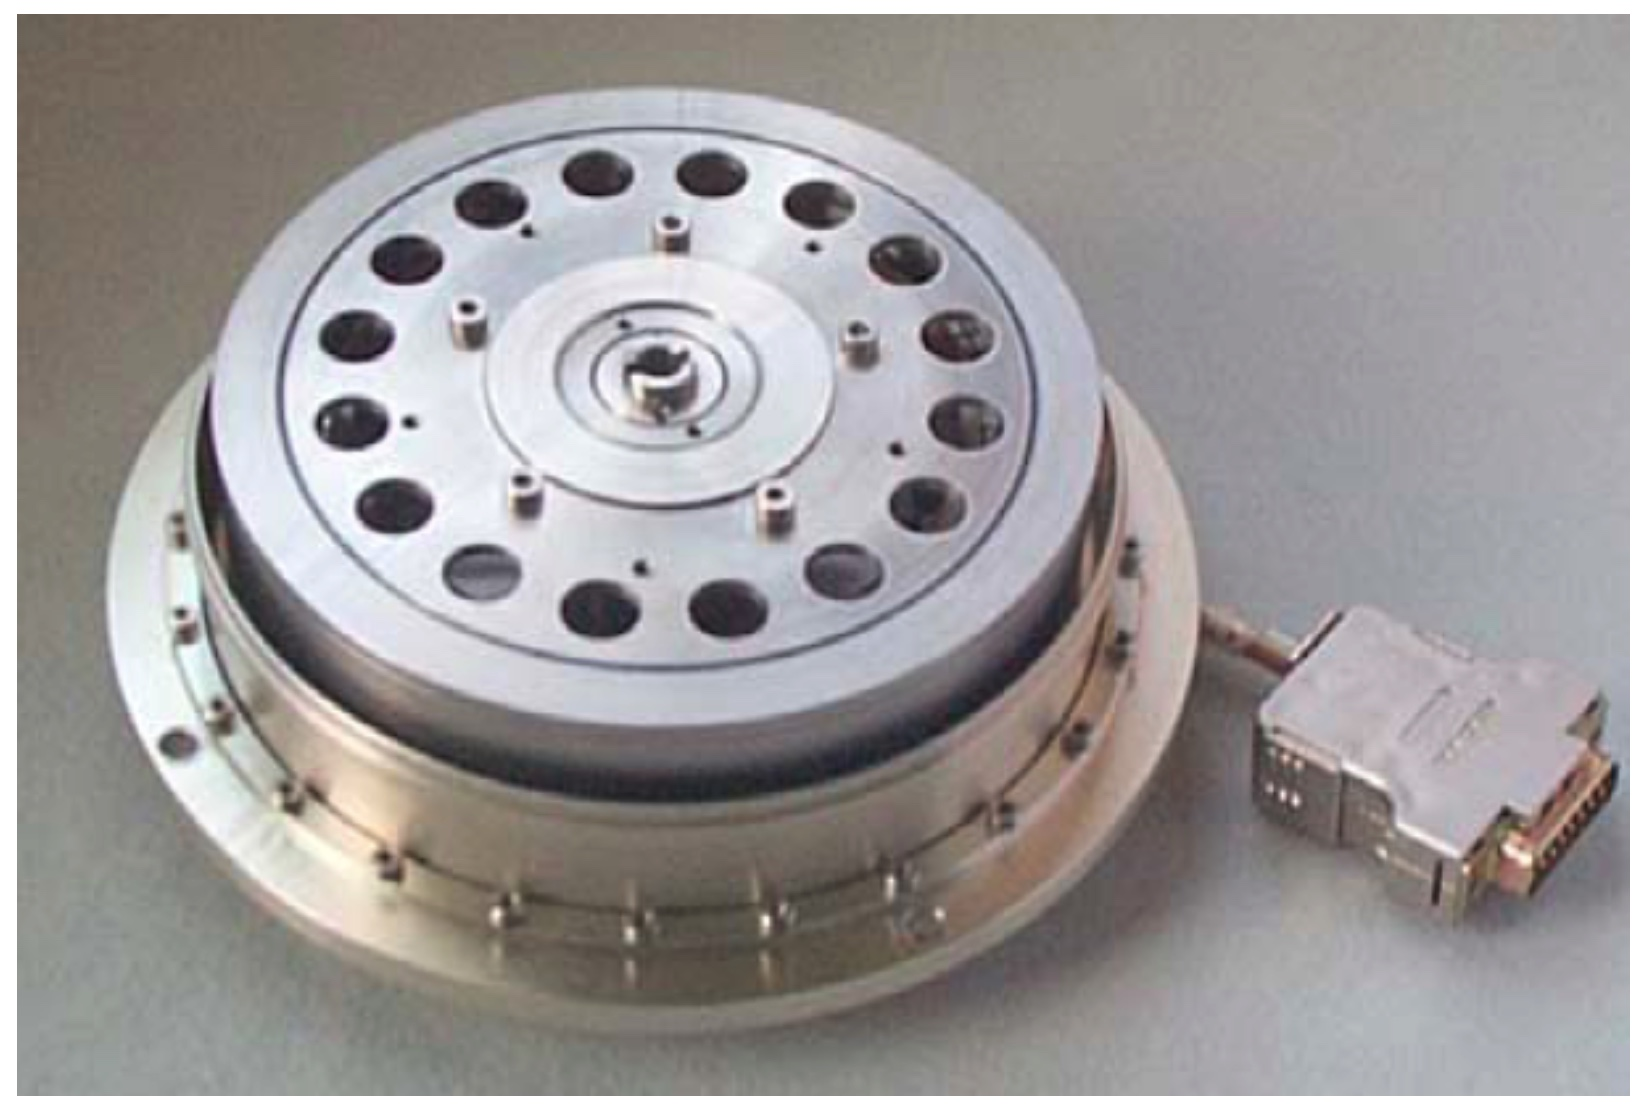
\includegraphics[width=0.5\textwidth]{images/image6.jpg}
\end{center}
\caption{Roue de réaction (carter ouvert) \label{fig6}}
\end{figure}
\fi

\subsubsection{Principe de fonctionnement d'une roue de réaction}

\ifprof
\else

Dans un premier temps, on s'intéresse à l'action d'une seule roue de
réaction, d'axe \couple{G_r}{\vect{y}}. On note :

\begin{itemize}
\item $\vect{\Omega}(R_e/R_s)=\omega_r\vect{y}$ le vecteur vitesse de rotation instantanée de la roue $R_r$ par rapport au
  satellite $R_s$, où $\omega_r(t)=\dot{\theta}_r(t)$ désigne la dérivée temporelle de l'angle de la rotation
  relative de la roue par rapport au satellite;
\item $\vect{\Omega}(R_s/R_g)=\Omega_x\vect{x}+\Omega_y\vect{y}+\Omega_z\vect{z}$
  le vecteur vitesse de rotation instantanée du satellite $R_s$ par rapport au
  référentiel géocentrique $R_g$ ;
\item $m_r$ la masse de la roue;
  
\item $G_r$ le centre d'inertie de la roue, situé sur l'axe de celle-ci;
  
\item $
I(G_r,R_r)=
\left(
\begin{array}{ccc}
I_{\text{rx}} & 0 & 0 \\ 
0 & I_{\text{ry}} & 0 \\ 
0 & 0 & I_{\text{rz}}
\end{array}
\right)_{\triplet{\vect{x}}{\vect{y}}{\vect{z}}} 
$
 la matrice d'inertie de la roue, avec $I_{\text{rx}}<I_{\text{ry}}$ et $I_{\text{rz}}<I_{\text{ry}}$.
  
\end{itemize}

Les actions mécaniques qui s'exercent sur la roue sont :

\begin{itemize}
\item l'action de la Terre~modélisée par: $
\torseur{\T\left(\text{Terre}\to \text{roue}\right)}=\torseurLigne{G_r}{-\mathcal{G}\dfrac{Mm_r}{\left(R+h\right)^2}\vect{Z}}{\vect{0}}$;   
\item l'action de la liaison pivot supposée parfaite entre la roue et le
  satellite~: 
$\torseur{\T\left(\text{satellite}\to \text{roue}\right)}=\torseurLigne{G_r}{\vect{F_l}(t)}{\vect{C_l}(t)} $;
  \item l'action du stator du moteur (lié au satellite) sur le rotor du moteur (lié à la roue)~modélisé par~:
  $\torseur{\T\left(\text{stator}\to \text{rotor}\right)}=\torseurLigne{G_r}{\vect{0}}{\left(C_m(t)-C_f(t)\right)\vect{y}}
$.
\end{itemize}

où $C_{m}$ désigne le couple moteur, et $C_{f}$ un
couple résistant. Comme l'ensemble est lubrifié, le couple résistant est
en fait un couple de frottement fluide $C_f(t)=f\cdot \omega_r(t)$ où le coefficient de frottement
\emph{f} est supposé connu avec précision.
\fi


\question{\label{q_13}}\textit{
  En supposant que les composantes $\left(\Omega_x,\Omega_y,\Omega_z\right)$ et leurs dérivées temporelles sont
  négligeables devant $\omega_r(t)$ et $\dot{\omega}_r(t)$ respectivement, déduire de l'application du
  théorème du moment dynamique l'équation scalaire du mouvement vérifiée
  par $\omega_r(t)$. Grâce à cette équation, exprimer, en fonction de $I_{ry}$ et $\dot{\omega_r}(t)$, le moment exercé par la roue sur le satellite.}
\ifprof
\begin{corrige}
\textbf{On isole la roue.}

\textbf{Bilan des actions mécaniques} :
\begin{itemize}
\item l'action de la Terre : $
\torseur{\T\left(\text{Terre}\to \text{roue}\right)}=\torseurLigne{G_r}{-\mathcal{G}\dfrac{Mm_r}{\left(R+h\right)^2}\vect{Z}}{\vect{0}}$;   
\item l'action de la liaison : 
$\torseur{\T\left(\text{satellite}\to \text{roue}\right)}=\torseurLigne{G_r}{\vect{F_l}(t)}{\vect{C_l}(t)} $;
  \item l'action du stator sur le rotor :
  $\torseur{\T\left(\text{stator}\to \text{rotor}\right)}=\torseurLigne{G_r}{\vect{0}}{\left(C_m(t)-C_f(t)\right)\vect{y}}
$ avec $C_f (t)=f \omega_r(t)$.
\end{itemize}

\textbf{Calcul du moment dynamique :}
La rotation de la roue à réaction étant suivant $\vect{y}$, on va donc chercher $\vectmd{G_r}{\text{Roue}}{R_g}\cdot \vect{y}$ :

$\vectmd{G_r}{\text{Roue}}{R_g}\cdot \vect{y}$ 
$=\left[\dfrac{\dd \vectmc{G_r}{\text{Roue}}{R_g}}{\dd t}\right]_{R_g}\cdot \vect{y}$ 
$=\left[ \dfrac{\dd   \left( I_{\text{rx}} \Omega_x \vect{x}+  I_{\text{ry}}\left( \Omega_y + \omega_r \right) \vect{y}+  I_{\text{rz}}\Omega_z \vect{z} \right)}{\dd t}\right]_{R_g}\cdot \vect{y}$ 

$=\left[ \dfrac{\dd   \left( I_{\text{rx}} \Omega_x \vect{x}+  I_{\text{ry}}\left( \Omega_y + \omega_r \right) \vect{y}+  I_{\text{rz}}\Omega_z \vect{z} \right)\cdot \vect{y}}{\dd t}\right]_{R_g}
\left( I_{\text{rx}} \Omega_x \vect{x}+  I_{\text{ry}}\left( \Omega_y + \omega_r \right) \vect{y}+  I_{\text{rz}}\Omega_z \vect{z} \right) +\left[ \dfrac{\dd   \vect{y}}{\dd t}\right]_{R_g}$ 
$ =I_{\text{ry}}\left( \dot{\Omega}_y + \dot{\omega}_r \right)$.

On a donc $\vect{C_l}(t)\cdot \vect{y} + C_m(t)-C_f(t)  =  I_{\text{ry}}\left( \dot{\Omega}_y + \dot{\omega}_r \right)$.


En tenant compte des hypothèses de la question et en remarquant que la liaison est une pivot parfaite d'axe $\vect{y}$ ($\vect{C_l}(t)\cdot\vect{y} = 0$), 
$C_m(t)-C_f(t) = I_{\text{ry}}\dot{\omega}_r$.


\end{corrige}
\else
\fi


\question{\label{q_14}}\textit{
  En partant de conditions initiales nulles, déterminer, en fonction de
  $I_y$ et $I_{\text{ry}}$, la relation entre la vitesse de rotation autour de l'axe $\vect{y}$ du
  satellite $\dot{\theta}(t)$ et la vitesse de rotation de la roue $\omega_r(t)$.}
  \ifprof
\begin{corrige}
On a vu (Question \ref{q_05}) que $I_y \ddot{\theta} = C_y^{\text{ext}}$ et 
$C_m(t)-C_f(t) = I_{\text{ry}}\dot{\omega}_r$. On a donc $- C_y^{\text{ext}} = C_m(t)-C_f(t)$ (à justifier...). 

En conséquences, $I_y \ddot{\theta} ^= - I_{\text{ry}}\dot{\omega}_r$. En intégrant, 
$I_y \dot{\theta} ^= - I_{\text{ry}}\omega_r$.
\end{corrige}
\else
\fi

  \ifprof
\else

   On utilisera pour cela l'une des équations déterminées dans la \textbf{question \ref{q_12}} en supposant pour simplifier que le torseur des actions mécaniques supplémentaires $\torseur{\T\left(\text{extérieur}\to \text{satellite}\right)}$
  ne comporte que l'action de la roue sur le satellite (on négligera
  donc toutes les autres actions, perturbatrices, exercées sur le
  satellite) et que les axes $\left(G,\vect{y}\right)$ et $\left(G_r,\vect{y}\right)$ sont confondus. On supposera de plus que
  le coefficient de frottement fluide, entre le stator et le rotor de la
  roue de réaction, est nul : $f=0$.

En réalité, le satellite est équipé de quatre roues de réaction de
caractéristiques identiques. L'une est orientée selon l'axe $\vect{x}$, deux autres
selon l'axe $\vect{y}$ et la quatrième est d'axe parallèle à $\vect{z}$. On rappelle que les axes $\vect{x}$, $\vect{y}$ et $\vect{z}$ sont les axes principaux d'inertie du satellite et sont concourants en G, centre d'inertie du satellite.
\fi

\question{\label{q_15}}\textit{ Justifier l'intérêt de disposer deux roues de réaction selon
  l'axe $\vect{y}$ plutôt qu'une seule.}
\ifprof
\begin{corrige}
\begin{itemize}
\item L’utilisation de 2 roues de réaction est l’illustration du principe de redondance
largement utilisé dans l’industrie qui consiste à sécuriser le fonctionnement d’un
système avec l’utilisation « en parallèle » de 2 solutions techniques identiques. En
effet, il serait dommage de perdre un satellite car une roue de réaction tombe en panne.
\item Le moment d’inertie selon l’axe $\axe{G_r}{\vy{}}$ étant le plus important, il est peut-être
privilégié de mettre en place 2 roues selon cet axe central d’inertie. En effet, du fait de
la différence des moments d’inerties des axes principaux, le composant de correction
d’attitude selon $\axe{G_r}{\vy{}}$ risque de faire office de fusible s’il n’est pas redondé.
\end{itemize}
\end{corrige}
\else
\fi

%\question{Qul estr}\label{Q6}
%
%Voici la \ref{Q6}
%
%\question{Qul estr}\label{Q7}
%
%Voici la \ref{Q7}


\subsubsection{Dimensionnement des roues de réaction}
\ifprof
\else

On s'intéresse maintenant au dimensionnement des roues de réaction. Le
cahier des charges associé est détaillé sur le tableau \ref{tab7}.

\begin{table}[!htb]
\begin{center}
\begin{tabular}{|c|c|}
\hline
Inertie de la roue autour de son axe &$I_a=\SI{4e-4}{kg.m^{2}}$\\ \hline
Hauteur maximale autorisée (selon l'axe de la roue) & $H=\SI{100}{m}$\\ \hline
Puissance maximale consommée autorisée par le moteur & $\mathcal{P}=\SI{1,5}{W}$\\ \hline
Masse & Minimale\\ \hline
\end{tabular}
\caption{Cahier des charges pour les roues de réaction \label{tab7}}
\end{center}
\end{table}



Chaque roue est conçue selon l'organisation suivante, détaillée sur la
\textbf{Figure \ref{fig8}} :

\begin{itemize}
\item  la roue proprement dite est un cylindre de rayon \emph{r} et de
  hauteur \emph{h} tous deux à déterminer ; elle est fabriquée en
  polyuréthane, de masse volumique $\rho_r=\SI{1140}{kg.m^{-3}}$ et de limite d'élasticité $\sigma_e=\SI{9}{MPa}$ qui caractérise la résistance de la roue à des actions mécaniques ;
\item   la roue est montée dans un carter en tôles d'acier d'épaisseur
 $e = \SI{2}{mm}$ et de masse volumique $\rho_c=\SI{7800}{kg.m^{-3}}$ , composé des éléments suivants :
  \begin{itemize}
  \item     un cylindre tubulaire de hauteur $H = 100 mm$ (encombrement
    maximal autorisé d'après le cahier des charges, mais hauteur
    nécessaire pour inclure le guidage et la motorisation de la roue) et
    de rayon extérieur $R$ à déterminer ;
  \item 
    deux plaques circulaires, de rayon $R$ à déterminer et
    d'épaisseur $e$, dont l'une est placée au-dessus et l'autre
    au-dessous du cylindre tubulaire ;
  \end{itemize}
\item  il existe un jeu radial $j=R-e-r=\SI{2}{mm}$ entre la roue et le carter.
\end{itemize}


\begin{figure}[!htb]
\begin{center}
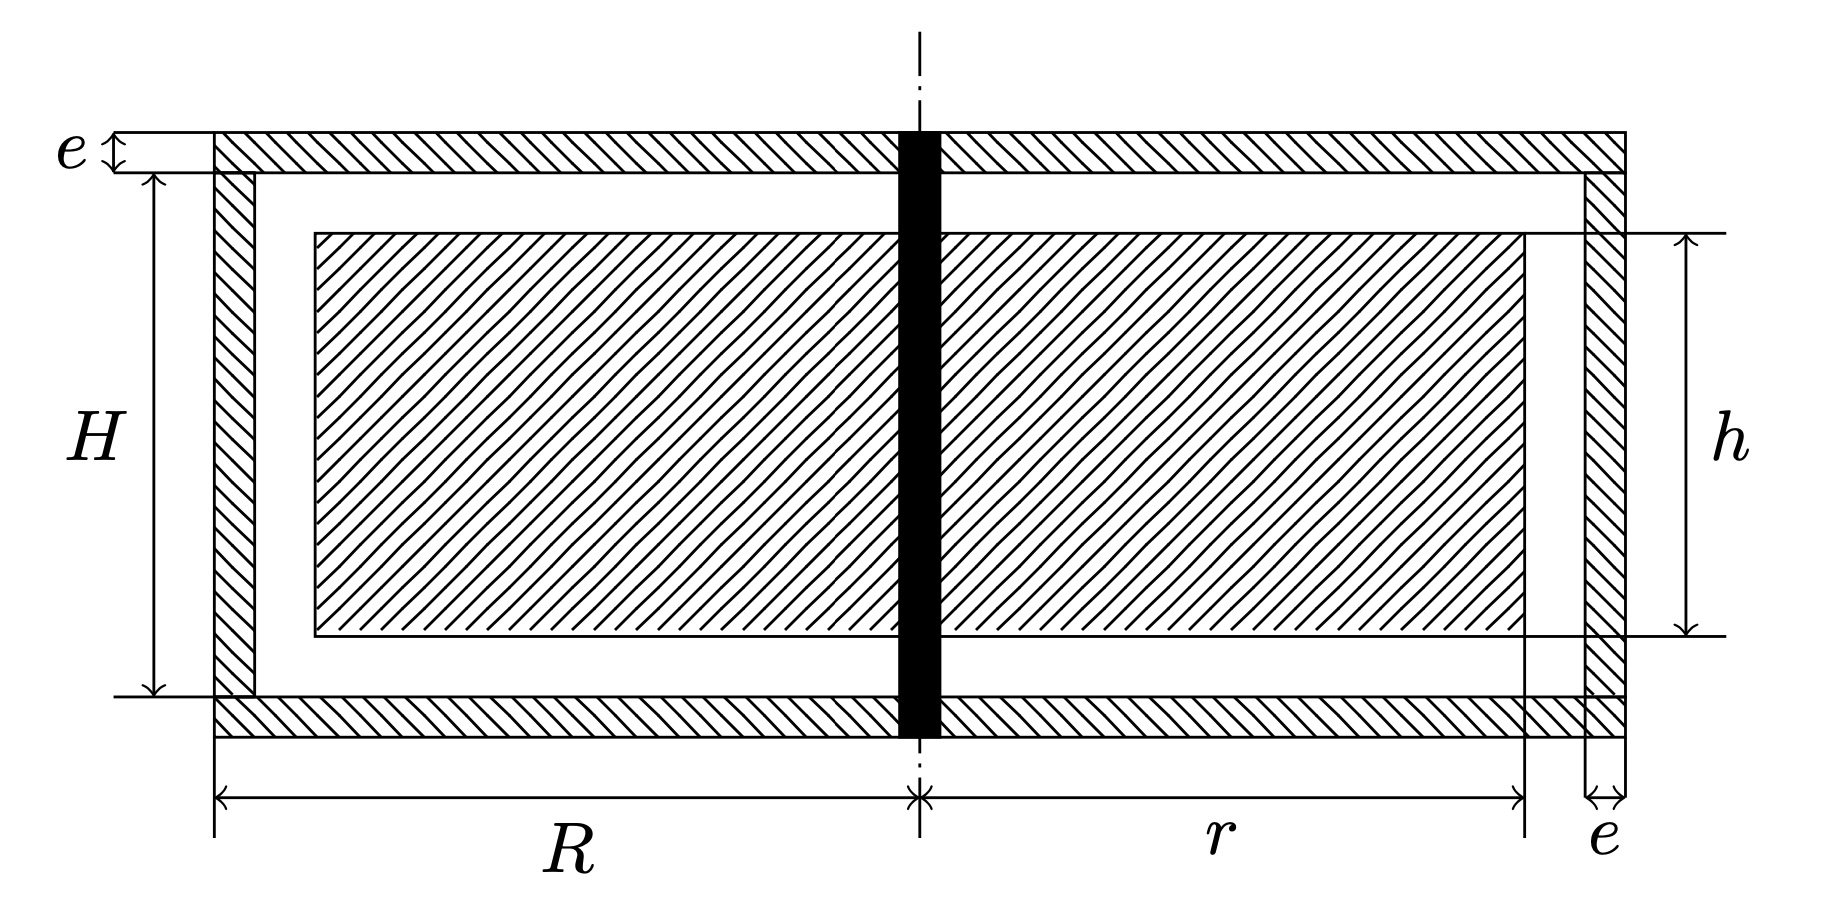
\includegraphics[width=0.6\textwidth]{images/image8.jpg}
\end{center}
\caption{Géométrie de la roue de réaction : le guidage en
rotation et la motorisation ne sont pas représentés, et les proportions
ne sont pas respectées \label{fig8}}
\end{figure}
\fi



\question{\label{q_16}}\textit{ Montrer que la masse totale de la roue de réaction (guidage et
motorisation exclus) peut s'écrire à l'ordre 1 en e et j comme :}
$$
m_t=\dfrac{2 I_a}{r^2}+2\pi\rho_c e r\left(r+H\right).
$$
\ifprof
\else
  On rappelle que le moment d'inertie $I_{\text{ac}}$ d'un cylindre plein, de masse $m_c$ et
  de rayon $r_C$, par rapport à son axe est $I_{\text{ac}}=\dfrac{1}{2}m_Cr_C^2$.
\fi

\ifprof
\begin{corrige}
Soient :
\begin{itemize}
\item $m_t$: la masse totale de la roue de réaction;
\item $m_r$ : la masse de la roue (cylindre en polyuréthane de rayon $r$ et de hauteur $h$);
\item $m_{\text{cyl}}$ : la masse du cylindre tubulaire du carter (tube en acier de masse volumique 
$\rho_c = \SI{7800}{kg.m^{-3}}$ de rayon extérieur $R$, d’épaisseur $e$ et de hauteur $H$);
\item $m_{\text{pla}}$ : la masse d’une plaque du carter (cylindre en acier de rayon $R$ et d’épaisseur $e$).
\end{itemize}
On trouve aisément la relation suivante : $m_t = m_r + m_{\text{cyl}}+2m_{\text{pla}}$.

Il est rappelé que le moment d’inertie d’un cylindre plein de masse $m_c$ et de rayon $r_c$ par
rapport à son axe d’inertie est $I_a = \dfrac{1}{2} m_c r_c^2$. On applique cette relation à la roue, aussi on en
déduit : $m_r = \dfrac{2I_a}{r^2}$.

La masse du cylindre tubulaire est définie par la relation suivante : $m_{\text{cyl}} = \rho_c \pi \left( R^2 - \left(R-e\right)^2\right)H$. 

La masse d’une plaque du carter est définie par la relation suivante : $m_{\text{pla}} = \rho_c \pi R^2 e$.

Ainsi on en déduit la relation de la masse totale suivante : $m_t = \dfrac{2I_a}{r^2} + \rho_c \pi \left( R^2 - \left(R-e\right)^2\right)H +2 \rho_c \pi R^2 e = \dfrac{2I_a}{r^2} + \rho_c \pi \left( 2R^2 e + \left(2eR-e^2\right)H\right)$.


Le jeu radial au niveau du carter est défini par la relation $j=R-e-r \Rightarrow  R = j+e+r$.

On a donc 

$m_t  = \dfrac{2I_a}{r^2} + \rho_c \pi \left( 2\left( j+e+r\right)^2 e + \left(2e\left( j+e+r\right)-e^2\right)H\right)$ 

$ = \dfrac{2I_a}{r^2} + \rho_c \pi \left(e\left(e+2j+2r \right)H + 2\left(r^2 + \left( j+e\right)^2 +2r \left( j+e\right)\right) e\right)$ avec $e+2j <<2r$ et $\left(j+e\right)^2+2r\left(j+e\right)<< r^2$ (hypothèse de linéarisation à l’ordre 1 en $e$ et $j$).

Ainsi on trouve la relation demandée $m_t =  \dfrac{2I_a}{r^2}+2\rho c \pi e r \left(H+r\right)$.

\end{corrige}


\else
\fi


  
  
\question{\label{q_17}}\textit{Montrer que cette masse totale $m_{t}$ est minimale pour
  une valeur spécifique de $r$ que l'on déterminera à l'aide de l'abaque donnée sur le document réponse. Calculer la masse
 $ m_{t}$ ainsi que les dimensions $h$ et $R$ des différents composants de la roue de réaction.}

\ifprof
\begin{corrige}

\end{corrige}
\else
\fi

\ifprof
\else
La technologie de moteur à courant continu utilisée pour piloter la roue
de réaction impose que la vitesse de rotation ne peut excéder $\SI{2800}{
tr.min^{-1}}$. Par ailleurs, la vitesse de rotation doit
être telle que les actions liées aux effets centrifuges dans la roue ne
causent pas la rupture du matériau ; par sécurité, on impose que la
contrainte maximale dans la roue ne dépasse pas la limite d'élasticité
du matériau :
$$
\sigma=\dfrac{7}{16}\rho_r\omega_r^2 r^2\leq \sigma_e
$$
\fi


\question{\label{q_18}}\textit{Quelle est, en définitive, la vitesse de rotation maximale (en
  $\SI{}{tr.min^{-1}}$) à laquelle pourra tourner la roue de
  réaction? En déduire, à l'aide du cahier des charges du tableau \ref{tab7},
  le couple moteur maximal $C_m(t)$ autorisé, ce qui permettra au final de
  choisir le moteur le plus adapté pour piloter la roue de réaction.}
\ifprof
\begin{corrige}

Afin d’éviter la rupture de la roue en polyuréthane (de limite d’élasticité $\sigma_e = \SI{9}{MPa}$ ), il est
imposé que la contrainte maximale ne soit pas dépassée dans le cas où les effets centrifuges
constituent le cas dimensionnant.
Ainsi, la relation suivante doit être respectée :
$\sigma = \dfrac{7}{16}\rho_r \omega_r^2r^2 \leq \sigma_e =\SI{9}{MPa}$ 
$\Longleftrightarrow \omega_r^2 \leq \dfrac{16 \sigma_e}{7\rho_r r^2}$
$\Longleftrightarrow \omega_r^2 \leq \dfrac{16\times 9\times 10^{6}}{7\times 1140\times 0,044^2}$
$\Longleftrightarrow \omega_r \leq \SI{3053}{rad.s^{-1}}$


On en déduit alors $N_{\text{r max}}=\dfrac{30\times 3053}{\pi}$.

Ainsi, le critère dimensionnant la vitesse de rotation de la roue est le choix de technologie
effectué et non les actions liées aux effets centrifuges.
D’après le Cdcf la puissance maxi consommée autorisée est $P_{\text{Max}}=\SI{1,5}{W}$. Or la vitesse de
rotation maximale est de \SI{2800}{tr.min^{-1}}. Ainsi on en déduit le couple maximal

$$
C_{m\text{Max}}(t)=\dfrac{30 P_{\text{Max}}}{\pi N} = \dfrac{1,5\times 30}{\pi \times 2800} = \SI{0,0051}{Nm}
$$

\end{corrige}
\else
\fi


\section{Contrôle d’attitude du satellite \label{sec:3}} \label{partieIII}
\begin{obj}
L’objectif de cette partie est de mettre en place une loi de commande permettant d’asservir les
positions angulaires du satellite à des positions de référence. Dans les parties \autoref{sec:3:A}, \autoref{sec:3:B} et \autoref{sec:3:C},
il s’agira de déterminer le régulateur qui assure les performances de la chaîne d’asservissement.
Dans la partie \autoref{sec:3:D}, il s’agira de vérifier si la loi de commande déterminée permet de respecter
les contraintes imposées à l’actionneur : couple maximal et vitesse maximale qu’il peut réaliser.
Dans le cas général, les lois de commande développées nécessitent une approche multivariable (trois
axes), le cadre de ce sujet se restreint uniquement aux mouvements de tangage, soit à la rotation
d’angle $\theta$  autour de l’axe $\vect{y}$. Les modèles utilisés ont été établis en adoptant $\psi  =\phi = 0$.
\end{obj}

\ifprof
\else

On rappelle que dans le mode de fonctionnement pointage fin (MNO) seuls les actionneurs par roues de réaction
et les magnétocoupleurs sont utilisés. Le cahier des charges partiel portant sur l’asservissement d’attitude est
détaillé dans le tableau de la \autoref{fig_09}. Ce cahier des charges doit être assuré même en cas d’un dépointage
initial qui sera modélisé comme condition initiale $\theta_0$ sur l’angle de tangage $\theta$. La consigne d’angle est notée $\theta_{\text{ref}}$ .

\begin{figure}[H]
\centering
\begin{tabular}{|p{.25\linewidth}|p{.35\linewidth}|p{.3\linewidth}|}
\hline
Chaîne d'asservissement & Ecart de pointage (en régimen permanent) & $| \Delta \theta | = | \theta_{\text{ref}}-\theta |\leq 0,04\degres$ \\
\cline{2-3}
& Pulsation de coupure $\omega_c à \SI{0}{dB}$ & $\SI{0,13}{rad.s^{-1}}$ \\ \cline{2-3}
& Marges de phase et de gain & $M\phi \geq 30\degres$ \\ \cline{2-3}
& & $MG \geq \SI{6}{dB}$ \\ \cline{2-3}
& Vitesse angulaire du satellite & $|\dot{\theta} | \geq  \SI{0,15}{\degres s^{-1}}$ \\ \hline
Actionneur à roue de réaction & Couple minimal & $|C|_{\text{max}} \leq \SI{0,005}{Nm}$ \\ \cline{2-3}
%& Couple minimal & $|C|_{\text{max}} \leq \SI{0,005}{Nm}$ \\ \hline
& Vitesse maximale & $|\Omega|_{\text{max}} \leq \SI{2800}{tr.min^{-1}}$ \\ \hline
Magnétocoupleurs & Couple maximal & $|C|_{\text{max}} \leq \SI{0,0005}{N.m}$ \\ \hline
Dépointage initial & Valeur maximale & $|\Theta|_{0} \leq \SI{20}{\degres}$ \\ 
\hline
\end{tabular}
%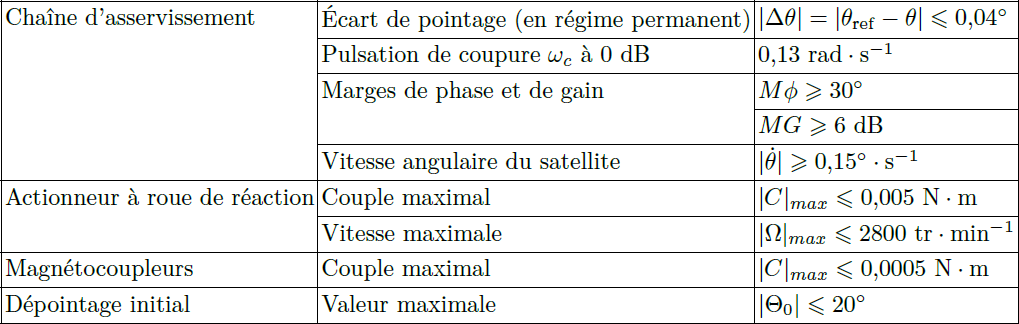
\includegraphics[width=\linewidth]{images/fig_09}
\caption{Cahier des charges pour la chaîne d’asservissement \label{fig_09}}

\end{figure}

L’architecture de contrôle d’attitude du satellite est représentée sur la \autoref{fig_10}. Dans le cas général, la loi de
commande utilise la mesure de la position angulaire du satellite et une estimation de sa vitesse. Dans le mode
de pointage fin, les actionneurs sont les roues de réaction qui fournissent un couple $C_{\text{roue}}$ conformément à un
couple de consigne $C_{\text{piloté}}$ demandé par la loi de commande. Le satellite est aussi soumis :
\begin{itemize}
\item à des couples perturbateurs sinusoïdaux de pulsations $\omega_0$ et $2\omega_{0}$ (avec $\omega_0 = \SI{0,001}{rad.s^{-1}}$) et d’amplitude,
dans le pire des cas, de $\SI{30e-6}{Nm}$;
\item à un couple constant d’amplitude $\SI{1e-6}{Nm}$.
\end{itemize}

\begin{figure}[H]
\centering
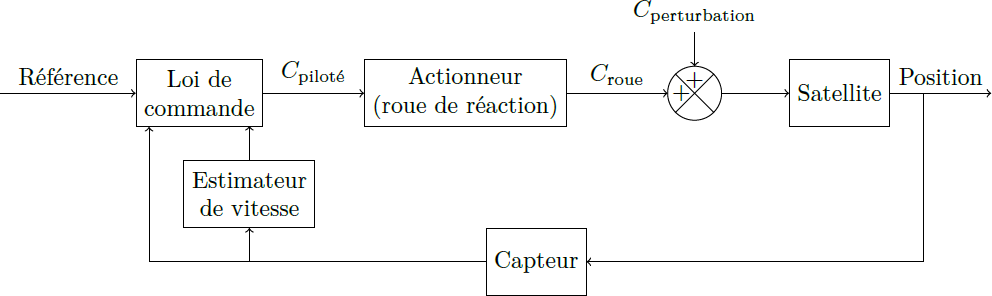
\includegraphics[width=.8\linewidth]{images/fig_10}
\caption{Architecture du système SCAO \label{fig_10}}
\end{figure}

Dans tous les modèles utilisés dans la suite, les angles sont exprimés en radians.

\fi

\subsection{\label{sec:3:A} Choix d’un modèle de commande et analyses préliminaires}

\ifprof
\else


La figure \autoref{fig_11} montre la chaîne de régulation (monoaxe) où $H(p)$, $A(p)$ et $B(p)$ sont les fonctions de transfert
modélisant respectivement le satellite, la roue de réaction et le capteur. On suppose dans un premier temps que
l’actionneur et le capteur ont tous deux un gain statique unitaire mais sont affectés d’un retard pur : \SI{100}{ms}
pour la roue de réaction et \SI{700}{ms} pour les capteurs stellaires. La fonction de transfert du satellite est obtenue à
partir des relations obtenues à la question \ref{q_8} ; et au regard de la bande passante souhaitée, on admettra qu’elle
peut être approchée par la fonction $H(p)$ donnée ci-dessous. Ainsi, les fonctions de transfert correspondant aux
différents éléments de la chaîne d’asservissement sont :
$$
H(p)=\dfrac{0,028}{p^2} 
\quad \quad 
A(p)=A_r (p) e^{-0,1p}\simeq \dfrac{1}{1+\dfrac{1}{0,87}p}e^{-0,1 p} 
\quad \quad 
B(p)=e^{-0,7p}
$$


Enfin, le correcteur représenté par la fonction de transfert $C(p) = R(p) F(p)$ est le produit de deux termes :
\begin{itemize}
\item $R(p)$ correspond à un régulateur de type PID (proportionnel, intégral, dérivé), qu’il s’agira de déterminer
dans la suite ;
\item $F(p)$ est la fonction de transfert d’un filtre de type passe-bas. Il a comme objectif de réduire le gain du système
en haute fréquence afin de ne pas exciter les modes oscillants (l’analyse de l’influence de ces modes est hors
du cadre de cette étude). Cette fonction de transfert sera approchée par la forme suivante 
$F(p) = \dfrac{1}{1 + 1,5p}$ (en pratique, ces filtres sont d’ordre 2).
\end{itemize}
\fi

\question{\label{q_15}}\textit{La figure du document réponse donne le diagramme de Bode de la fonction $A_r(p)H(p)F(p)$. Tracer
directement sur cette figure les diagrammes asymptotiques associés à cette fonction (document réponse à rendre
avec la copie).}
\ifprof
\begin{corrige}
Les pentes des asympotes sont données par le tableau suivant. 
\begin{figure}[H]
\centering
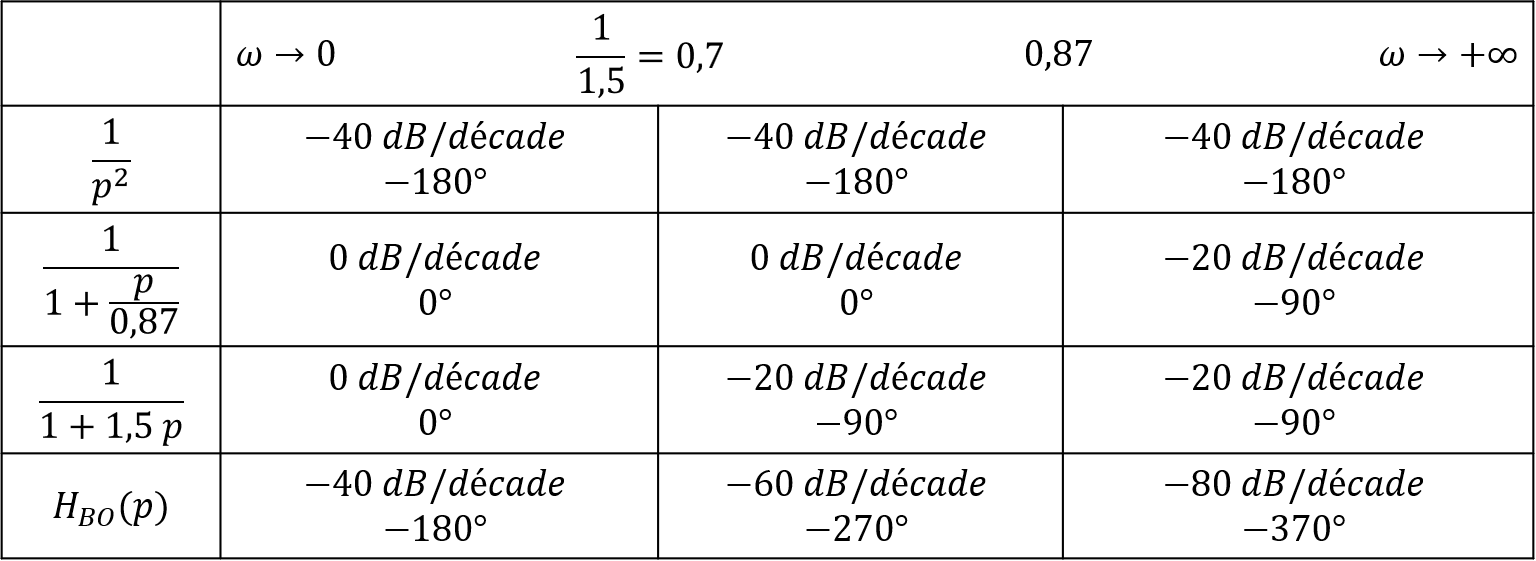
\includegraphics[width=.8\linewidth]{images/cor_q15}

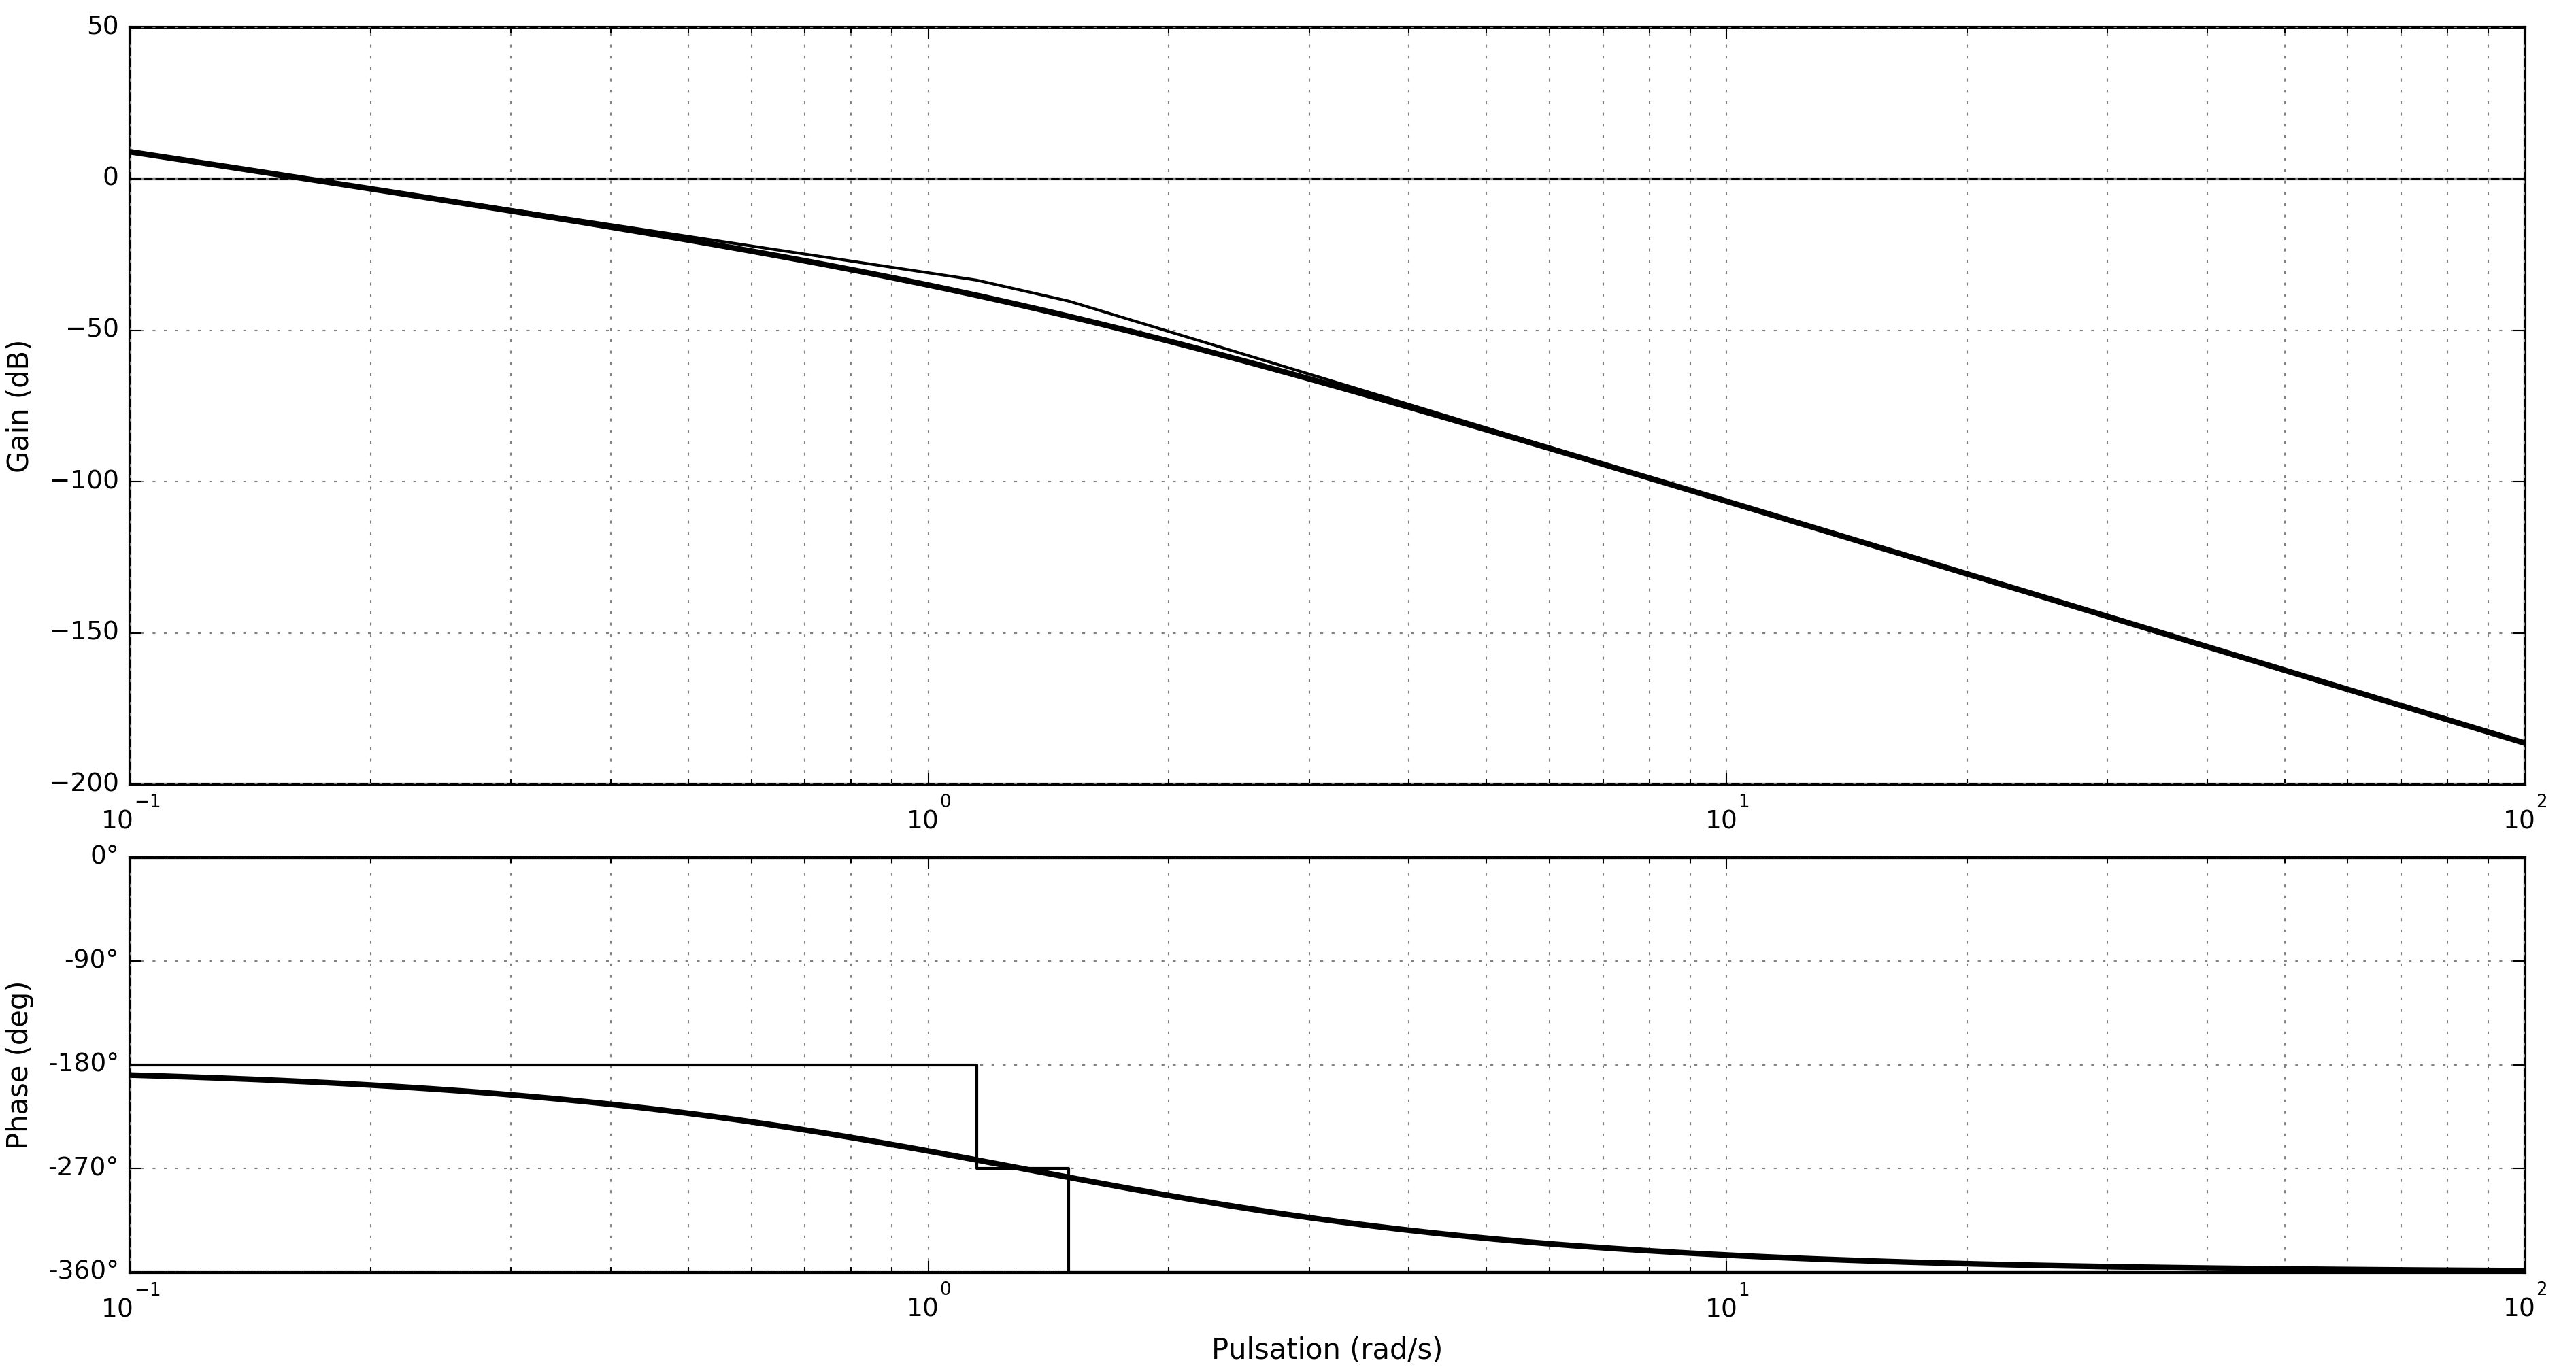
\includegraphics[width=.8\linewidth]{images/cor_q15_bode}
%\caption{Architecture du système SCAO \label{fig_10}}
\end{figure}

De plus, en basse fréquence, lorsque 
$\omega << \SI{0,1}{rad.s^{-1}}$, 
$H_{\text{BO}}(p)\simeq \dfrac{0,028}{p^2}$. 
On a donc  en $\omega = \SI{0,01}{rad.s^{-1}}$, $G_{\text{dB}}(0,01)\simeq 20\log \left(\dfrac{0,028}{0,01^2}\right)\simeq \SI{50}{dB}$.


\end{corrige}
\else
\fi

\question{\label{q_16}}\textit{En prenant $R(p) = 1$, préciser la fonction de transfert en boucle ouverte et tracer les diagrammes de
Bode réels (5 ou 6 points judicieusement choisis suffisent pour ces tracés) sur la figure B. Au regard des tracés
effectués, justifier que des corrections proportionnelle ou proportionnelle-intégrale ne permettent pas d’assurer
le cahier des charges escompté.}
\ifprof
\begin{corrige}
On a $\text{FTBO}(p)=F(p)A(p)H(p)B(p)=\dfrac{1}{1 + 1,5p} \dfrac{1}{1+\dfrac{1}{0,87}p}e^{-0,1 p}  \dfrac{0,028}{p^2} e^{-0,7p}$. Il s'agit donc d'ajouter le retard $e^{-0,8 p}$.

Le gain du retard est unitaire. Il ne change donc pas le diagramme de gain.
Le déphase ajouté par le retard est de $-0,8\omega $. 
On << descend >> donc la phase des valeurs suivantes. 

\begin{figure}[H]
\centering
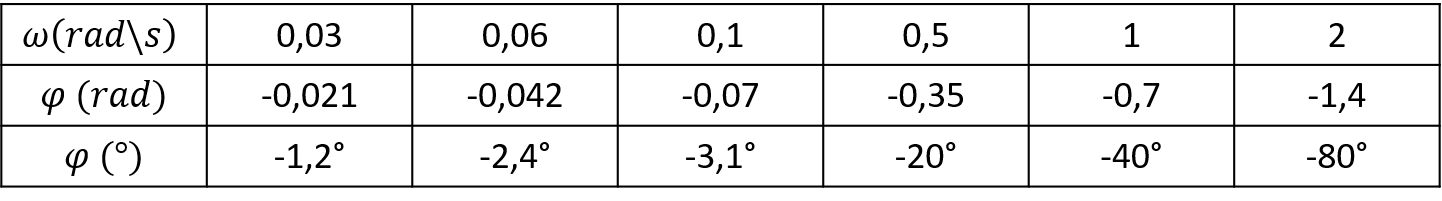
\includegraphics[width=.8\linewidth]{images/cor_q16}
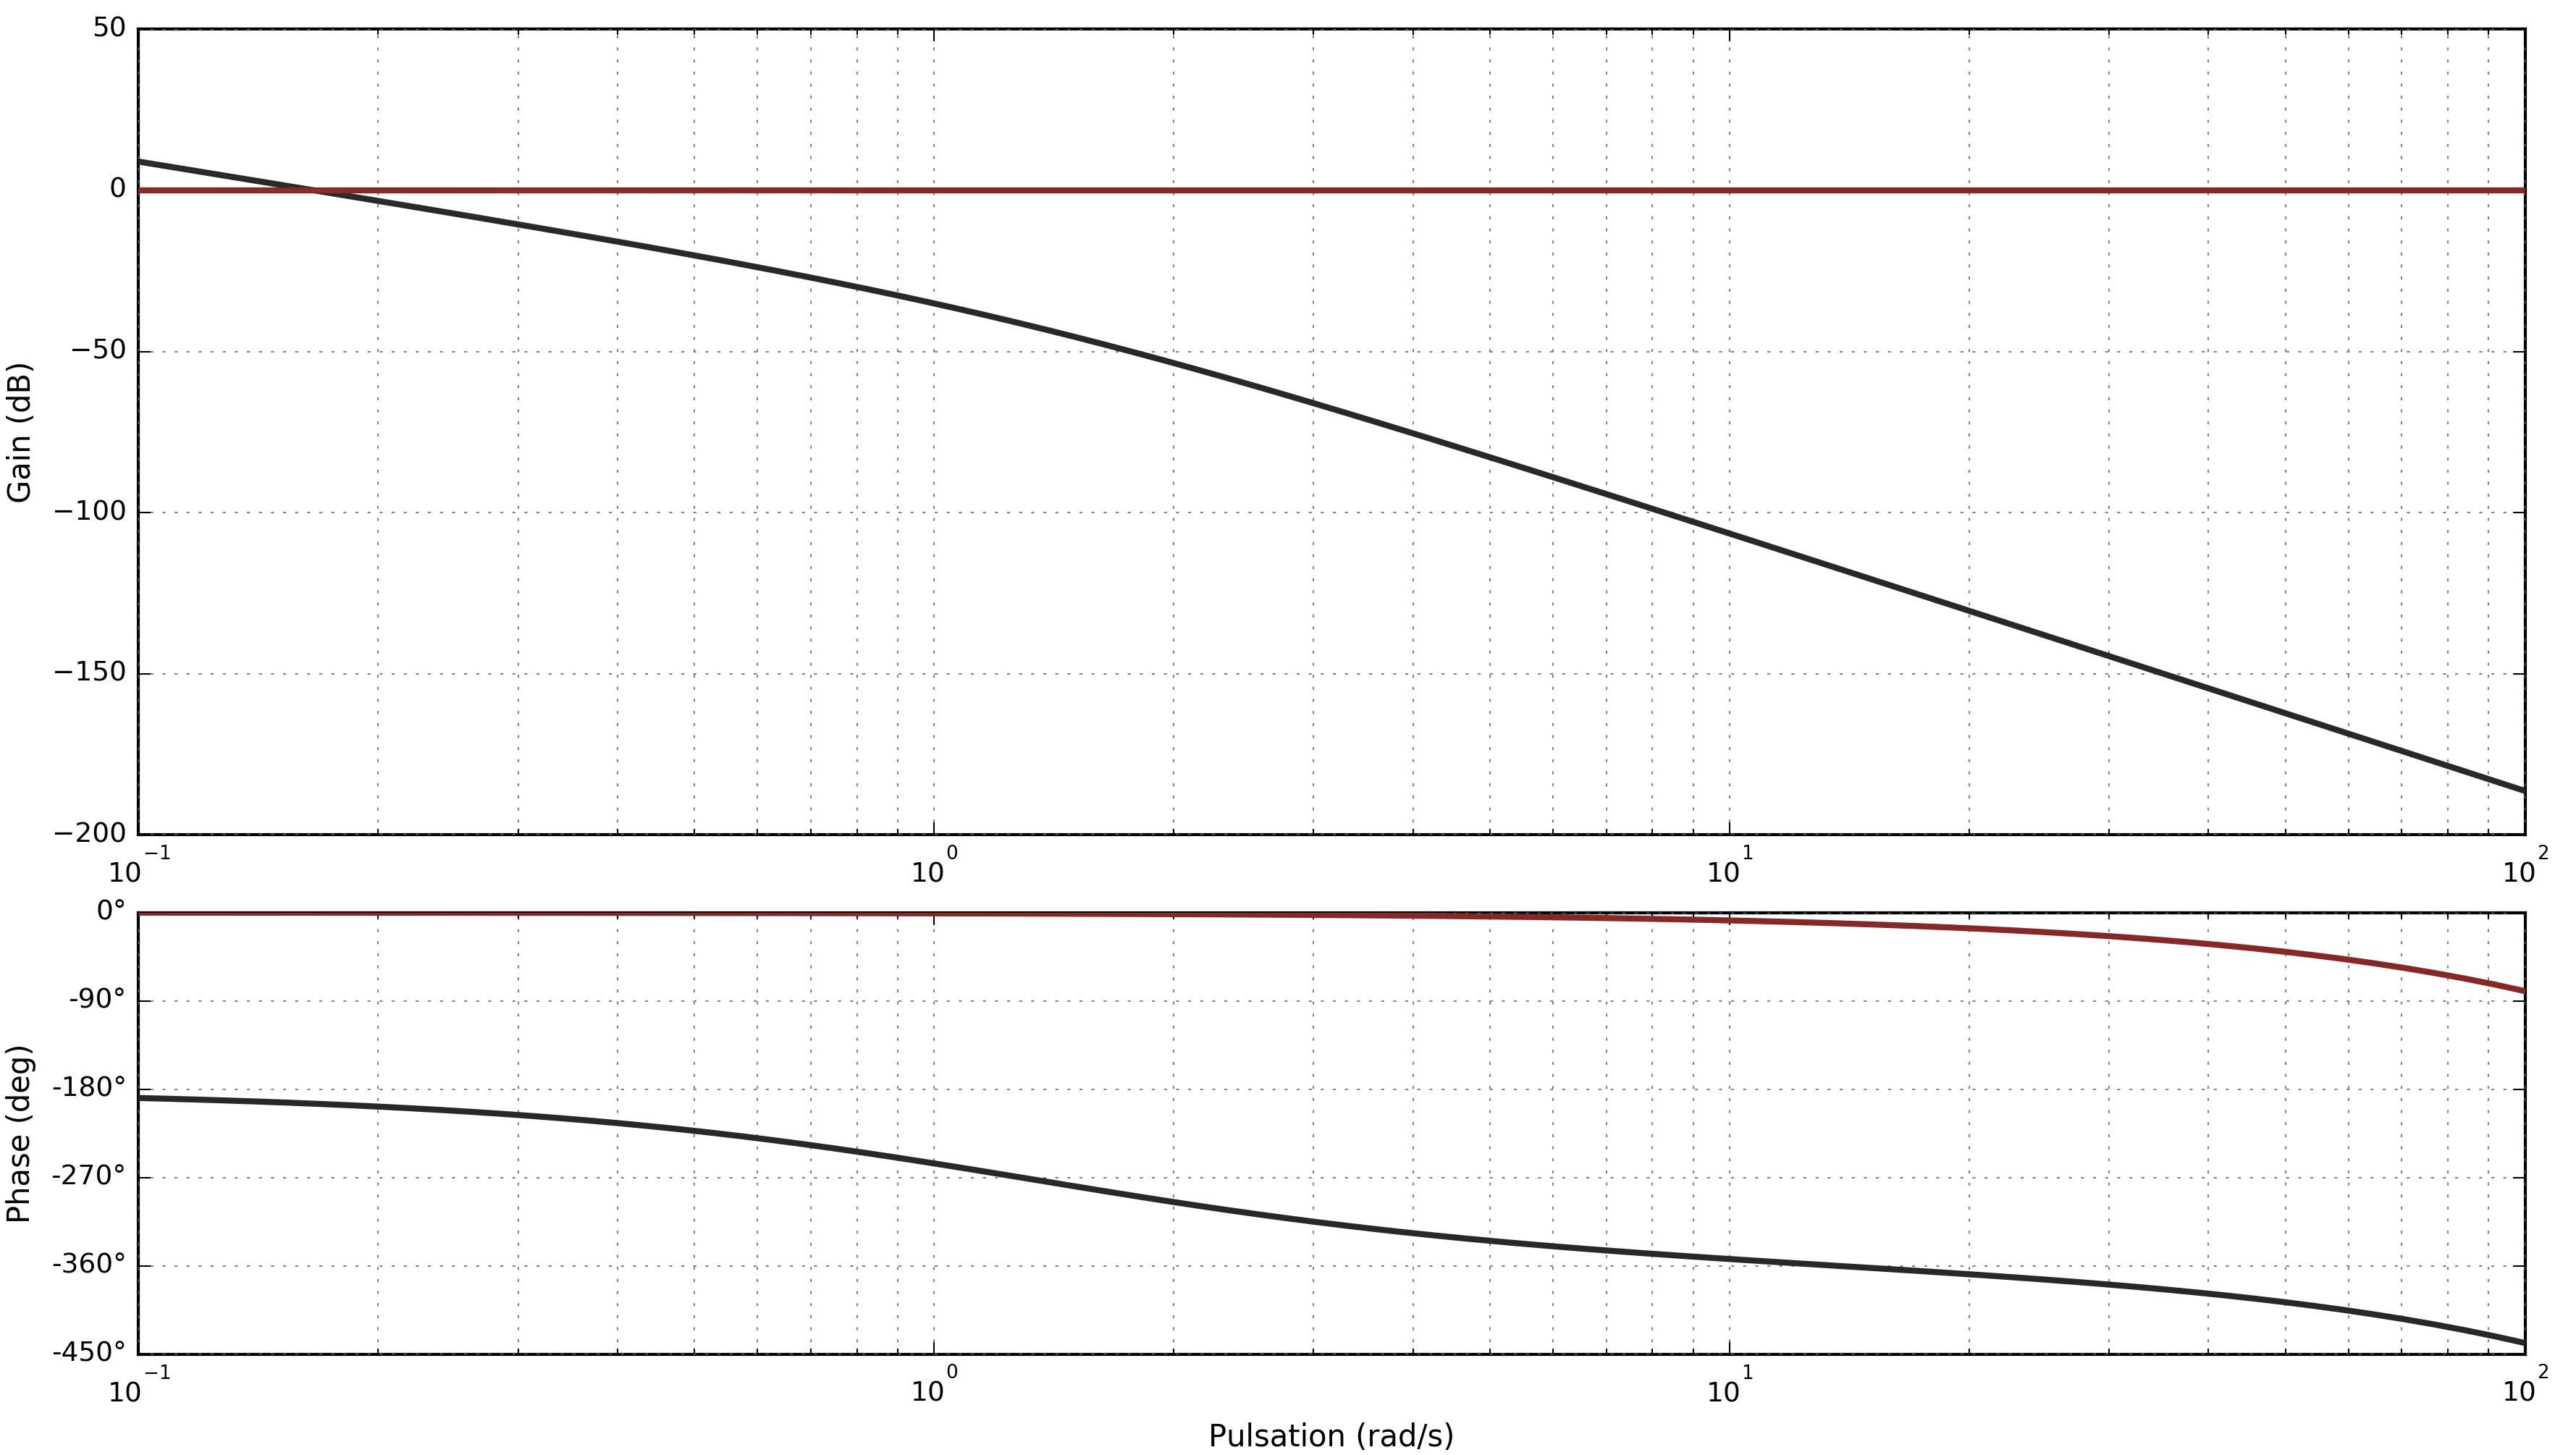
\includegraphics[width=.8\linewidth]{images/cor_q16_bode}
%\caption{Architecture du système SCAO \label{fig_10}}
\end{figure}

Cahier des charges :
\begin{itemize}
\item écart de pointage : avec un double intégrateur, le système est précis pour une entrée échelon -- exigence respectée;
\item pulsation de coupure à $\SI{0}{dB}= \SI{0,13}{rad.s^{-1}}$ -- exigence respectée (et réglable avec des correcteurs P et PI);
\item marge de phase : avec un système de classe 2, la phase est forcément inférieure à $-\SI{180}{\degres}$ -- exigence qui ne pourra pas être respectée avec un P ou un PI;
\item marge de gain : si la marge de phase n'est pas respectée, on ne pourra pas stabiliser le système...
\end{itemize}

\end{corrige}
\else
\fi


\question{\label{q_17}}\textit{En déduire les conditions sur le module et l’argument de $R(j\omega)$ pour assurer la pulsation de coupure et
la marge de phase demandées par le cahier des charges associé au modèle nominal.}
\ifprof
\begin{corrige}
En utilisant la BO non corrigée, on mesure :
\begin{itemize}
\item $\omega_{\SI{0}{dB}} = \SI{0,16}{rad.s^{-1}}$;
\item $M_{\varphi}=-\SI{25}{\degres}$
\end{itemize}
Le cahier des charges demande 
\begin{itemize}
\item $\omega_{\SI{0}{dB}} = \SI{0,13}{rad.s^{-1}}$;
\item $M_{\varphi}\geq \SI{30}{\degres}$, il faut donc que $\arg\left(R(j\omega_{\SI{0}{dB}}) \right)=45\degres$.
\item $M_{G}\geq \SI{6}{dB}$.
\item Dans ces conditions, il faudrait déterminer la pulsation pour laquelle la phase vaut $-180\degres$ puis ajuster le gain.
\end{itemize}
\end{corrige}
\else
\fi


\ifprof
\else

\begin{figure}[H]
\centering
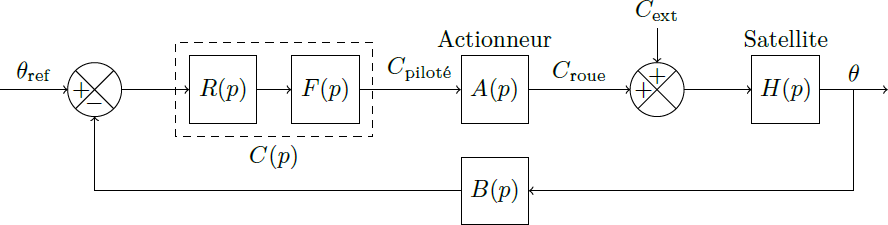
\includegraphics[width=.8\linewidth]{images/fig_11}
\caption{Schéma-bloc de la boucle d’asservissement d’attitude \label{fig_11}}
\end{figure}

\fi




\subsection{\label{sec:3:B} Analyse des contraintes sur la loi de commande}

\ifprof
\else

L’objet de cette partie est de déterminer les contraintes que doit vérifier le régulateur en vue d’assurer les
exigences de précision lorsque le procédé est soumis aux couples perturbateurs sinusoïdaux, c’est-à-dire de la
forme 
$c_{\text{ext}} = C_{00}\sin(\omega_0 t)$ et 
$c_{\text{ext}} = C_{01} \sin(2\omega_0t)$, 
dont les caractéristiques, amplitude et pulsation, sont données
précédemment : $C_{00} = C_{01} = \SI{30e-6}{N.m}$  et $\omega_0 = \SI{0,001}{rad.s^{-1}}$.
\fi


\question{\label{q_18}}\textit{En prenant une consigne $\theta_{\text{ref}} = 0$, déterminer la fonction de transfert $T(p) = \dfrac{\theta(p)}{C_{\text{ext}}(p)}$ entre les couples perturbateurs $C_{\text{ext}}(p)$ et la position $\theta(p)$ et l’exprimer à partir des fonctions de transfert de la \autoref{fig_11}.}
\ifprof
\begin{corrige}
On a $T(p)=\dfrac{H(p)}{1+H(p)B(p)A(p)C(p)}$ ou encore $T(p)=\dfrac{H(p)}{1+H(p)B(p)A(p)F(p)R(p)}$
\end{corrige}
\else
\fi

\question{\label{q_19}}\textit{En utilisant les approximations fréquentielles 
$||T_{\text{bo}}(j\omega)||>>1$ et
$||T_{\text{bo}}(j\omega)||<<1$
où $T_{\text{bo}}(p)$ est la fonction
de transfert en boucle ouverte, montrer que dans l’intervalle des pulsations des couples perturbateurs, 
on peut écrire : 
$||T(j\omega)||\simeq \dfrac{1}{|| R\left(j\omega\right) F\left(j\omega\right) A\left(j\omega\right) B\left(j\omega\right)|| }$. 
 Justifier que cette relation peut encore être simplifiée selon la formulation :
 $||T(j\omega)||\simeq \dfrac{1}{|| R\left(j\omega\right)||}$.}

\ifprof
\begin{corrige}
Pour des pulsations comprises entre $\SI{0,001}{rad.s^{-1}}$ et $\SI{0,002}{rad.s^{-1}}$, la FTBO tend vers $H(p)R(p)$.
Le gain est de la FTBO y est supérieur à \SI{40}{dB}. On peut donc considérer que 
$||T(j\omega)||\simeq \dfrac{||H\left(j\omega\right)||}{|| H\left(j\omega\right) R\left(j\omega\right) F\left(j\omega\right) A\left(j\omega\right) B\left(j\omega\right)|| } = \dfrac{1}{|| R\left(j\omega\right) F\left(j\omega\right) A\left(j\omega\right) B\left(j\omega\right)|| }$.

Or, $||F\left(j\omega\right) A\left(j\omega\right) B\left(j\omega\right)|| \simeq 0$ entre  entre $\SI{0,001}{rad.s^{-1}}$ et $\SI{0,002}{rad.s^{-1}}$; donc $||T(j\omega)||\simeq \dfrac{1}{|| R\left(j\omega\right)||}$.

\end{corrige}
\else
\fi

\question{\label{q_20}}\textit{Donner l’expression de l’amplitude de  l'évolution temporelle de $\theta(t)$, en fonction de 
de $|| R\left(j \omega\right)||$,  en réponse
au couple perturbateur sinusoïdal de pulsation $\omega_0$. En déduire la condition que doit vérifier $|| R\left(j \omega\right)||$ en vue de
satisfaire la précision d’écart de pointage, pour une consigne $\theta_{\text{ref}} = 0$, lorsque le satellite est soumis à ce couple
perturbateur. Reprendre cette analyse dans le cas du couple 
perturbateur de pulsation $2\omega_0$.}
\ifprof
\begin{corrige}
La perturbation étant sinusoïdale de la forme 
$c_{\text{ext}} = C_{00}\sin(\omega_0 t)$ on a 
$\theta(t)=K C_{00}\sin(\omega_0 t + \varphi)$ avec 
$K = \dfrac{1}{|| R\left(j\omega_0\right)||} $ et 
$\varphi = \arg\left( T(j\omega_0) \right)$.

D'après le cahier des charges, l'écart de pointage doit rester inférieur à $\SI{0,04}{\degres} = \SI{7e-4}{rad}$.
De plus, $C_{00}=C_{01}$; donc $K C_{00} <  \SI{7e-4}{rad} \Rightarrow K < \dfrac{7\times 10^{-4}}{30\times 10^{-6}} = \SI{23}{rad.N^{-1}m^{-1}}$ et $|| R\left(j\omega_0\right)|| > \SI{0,043}{Nmrad^{-1}}$.

\end{corrige}

\else
\fi

\subsection{\label{sec:3:C} Synthèse du régulateur}

Pour la synthèse du régulateur $C(p)$, on recherche une solution de la forme : $R(p)=K \dfrac{\left(1+\tau p\right)^2}{p}$.

\question{\label{q_21}}\textit{Déterminer la valeur de
$\tau$  permettant d’obtenir 
la marge de phase 
$M \phi = 30\degres$
 exigée par le cahier des charges.}
\ifprof
\begin{corrige}
On a $\arg{R(p)} = \arg{K}+ \arg{\left(1+\tau p\right)^2} - \arg{p}$
$ =-\dfrac{\pi}{2}  +2 \arctan\left(\tau \omega \right)$.

D'après la question \ref{q_17}, l'apport de phase ajouté doit être de \SI{55}{\degres} pour une pulsation de $ \SI{0,13}{rad.s^{-1}}$; donc $55=-90  +2 \arctan\left(\tau 0,13 \right) $ et $\tau = \tan \left(\dfrac{55+180}{2}\right) \dfrac{1}{0,13} = \SI{24,4}{s}$.
\end{corrige}
\else
\fi 



\question{\label{q_22}}\textit{En conservant la valeur de $\tau$ déterminée précédemment, 
calculer la valeur du gain $K$ qui assure la pulsation de coupure imposée par le cahier des charges.}
\ifprof
\begin{corrige}
On a $||T_{\text{bo}}(j\omega)||=||H(j\omega)B(j\omega)A(j\omega)F(j\omega)R(j\omega)||$
$=0,028 \dfrac{1}{\omega^2}\dfrac{1}{\sqrt{1+\dfrac{\omega^2}{0,87^2}}}\dfrac{1}{\sqrt{1+\omega^2 1,5^2}} K \dfrac{1+\tau^2\omega^2}{\omega}$.

Pour $\omega = \omega_{\SI{0}{dB}}=\SI{0,13}{rad.s^{-1}}$ et $\tau=\SI{24,4}{s}$; 
$||T_{\text{bo}}(j\omega_{\SI{0}{dB}})|| = 136,8 K$. On souhaite que le gain dB soit nul (et donc le module unitaire); donc $K= \dfrac{1}{136,8} = 0,0073$.
\end{corrige}
\else
\fi

\question{\label{q_23}}\textit{Vérifier si le régulateur déterminé permet d’assurer les conditions nécessaires à satisfaire les performances,
en termes d’écart de l’angle de pointage, lorsque le satellite est soumis aux variations sinusoïdales du couple
perturbateur.}
\ifprof
\begin{corrige}

Si on considère qu'en basses fréquences,  $||T(j\omega)||\simeq \dfrac{1}{|| R\left(j\omega\right)||}$.


$|| R\left(j\omega\right)|| = \left|\left| 0,073  \dfrac{\left(1+24,4 j \omega\right)^2}{j\omega}\right|\right|$
$=0,073  \dfrac{ \left|\left| 1+24,4 j \omega \right|\right| ^2}{ \left|\left| j\omega\right|\right|}$
$=0,073  \dfrac{ 1+24,4^2  \omega^2 }{ \omega}$

Pour une perturbation sinusoïdale, l'amplitude de $\theta$ est donnée par $||T(j\omega)|| C_{00}$.  D'où :
\begin{itemize}
\item pour $\omega = \SI{0,001}{rad.s^{-1}}$, $||T(j\omega)|| C_{00} = 0,14 \times 30 \times 10^{-6} = \SI{5.8e-6}{rad} = 0,0003\degres\leq 0,04\degres$;
\item pour $\omega = \SI{0,002}{rad.s^{-1}}$, $||T(j\omega)|| C_{00} = 0,27 \times 30 \times 10^{-6} = \SI{2,2e-5}{rad} = 0,0012\degres\leq 0,04\degres$.
\end{itemize}
%on a, 
% dans le pire des cas, $||T(0,002 j)|| = \dfrac{1}{\left|\left| 0,073  \dfrac{\left(1+24,4 j \omega\right)^2}{j\omega}\right|\right|} = \left(0,0073 \dfrac{1+24,4^2\times 0,002^2}{0,002}\right)^{-1/2} \simeq (3,6)^{-1} =0,28$. On a $0,28\times 30\times 10^{-6}=4,77\times 10^{-4} \degres<0,04\degres$.
%  ***(AN à vérifier))
%  
\end{corrige}
\else
\fi

\subsection{\label{sec:3:D} Validation de la loi de commande}
\begin{obj}
L’objectif de cette partie est de vérifier que les commandes issues du régulateur précédent ne
génèrent pas de contraintes excessives sur l’actionneur, en particulier que la vitesse maximale
et le couple maximal restent dans les « limites » de l’actionneur réalisé par la roue de réaction.
Cette vérification se fera d’une part vis-à-vis d’un dépointage initial et d’autre part vis-à-vis des
différents couples perturbateurs. Enfin, une modification de la loi de commande sera envisagée en
vue d’améliorer les performances.
\end{obj}

\subsubsection{\label{sec:3:D:1} Amélioration des performances vis-à-vis du dépointage initial}

\ifprof
\else

Pour cette analyse, on suppose que les conditions initiales correspondent à un dépointage de 20\degres, soit $\theta_0 = 20\degres$,
et que la consigne d’attitude est nulle $\theta_{\text{ref}}=0$. La \autoref{fig_12} montre le schéma qui sera utilisé pour cette analyse
où la condition initiale $\theta_0$ d’attitude est considérée comme un terme de perturbation constant.

\begin{figure}[H]
\centering
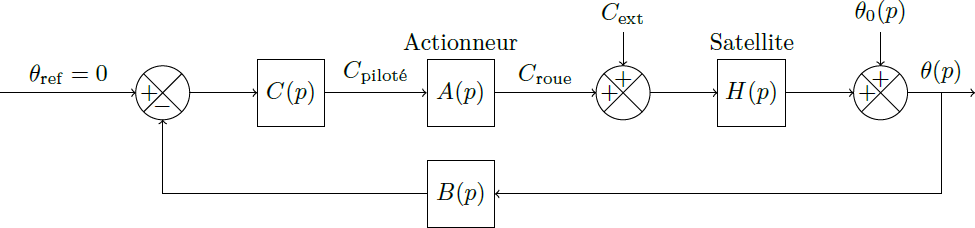
\includegraphics[width=\linewidth]{images/fig_12}
\caption{Schéma d’analyse pour la réponse aux conditions initiales \label{fig_12}}
\end{figure}
\fi

%\question{\label{q_24}}\textit{Déterminer $T_d(p)=\dfrac{C_{\text{piloté}}(p)}{\theta_0(p)}$ à partir des différentes fonctions de transfert de la \autoref{fig_12}. On note $c_{\text{pa}}(p)=c_{\text{piloté}}(t+\tau_1)$, avec $\tau_1 = \SI{0,7}{s}$. En déduire à partir de $T_d(p)$ l'expression de $\dfrac{C_{\text{pa}}}{\theta_0(p)}$.}% QUESTION ORIGINALE

\question{\label{q_24}}\textit{En considérant que  $\theta_{\text{ref}}=0$ et  $C_{\text{ext}}=0$, déterminer $T_d(p)=\dfrac{C_{\text{piloté}}(p)}{\theta_0(p)}$ à partir des différentes fonctions de transfert de la \autoref{fig_12}. On note $c_{\text{pa}}(t)=c_{\text{piloté}}(t+\tau_1)$, avec $\tau_1 = \SI{0,7}{s}$. En déduire à partir de $T_d(p)$ l'expression de $\dfrac{C_{\text{pa}}(p)}{\theta_0(p)}$.} % Question modifiée
\ifprof
\begin{corrige}
Dans les conditions énoncées : $C_{\text{piloté}}(p)=-\theta(p) B(p) C(p)$. De plus,$\theta(p)=\theta_0(p)+C_{\text{piloté}}(p) A(p) H(p)$. 
On a donc $C_{\text{piloté}}(p)=-\left( \theta_0(p)+C_{\text{piloté}}(p) A(p) H(p) \right) B(p) C(p)$.
En conséquences, $C_{\text{piloté}}(p)\left( 1+ A(p) H(p) B(p) C(p) \right)=- \theta_0(p) B(p) C(p)$.
Au final, $T_d(p)=\dfrac{C_{\text{piloté}}(p)}{\theta_0(p)} = -\dfrac{ B(p) C(p)}{ 1+ A(p) H(p) B(p) C(p)}$.


 On a $c_{\text{pa}}(t)=c_{\text{piloté}}(t+\tau_1)$ $\Leftrightarrow c_{\text{pa}}(t-\tau_1)=c_{\text{piloté}}(t) $ . En utilisant le théorème du retard, et en passant dans le domaine de Laplace, 
  $C_{\text{pa}}(p)e^{-\tau_1 p} =C_{\text{piloté}}(p)$. 
  
Or, $T_d(p)=\dfrac{C_{\text{piloté}}(p)}{\theta_0(p)}$; donc $T_d(p)=\dfrac{C_{\text{pa}}(p)e^{-\tau_1 p}}{\theta_0(p)}$.


\end{corrige}
\else
\fi

\question{\label{q_25}}\textit{En utilisant le théorème de la valeur initiale,
ou toute autre méthode de votre choix, déterminer littéralement
et numériquement $c_{\text{pa}}(0)$ en réponse à une condition initiale 
$\theta_0(t)=\Theta_0 \gamma(t)$ d'amplitude $\Theta_0 = 20\degres$. En
déduire $c_{\text{piloté}}(\tau_1)$. 
[Remarques : $\gamma(t)$ désigne l’échelon d’Heaviside d’amplitude 1. On admettra que la valeur déterminée est proche de la 
valeur maximale (en valeur absolue) de celle obtenue pour des cas d’utilisation
de filtres $F(p)$ d'ordre supérieur à~1.]}
\ifprof
\begin{corrige}

D'après la question précédente,  $C_{\text{pa}}(p) = T_d(p) \theta_0(p)  e^{\tau_1 p}$.

Par application du théorème de la valeur initiale, 

$c_{\text{pa}}(0) = \lim\limits_{p \to \infty} p T_d(p) \theta_0(p)  e^{\tau_1 p} $. Or $\theta_0(p) = \dfrac{\Theta_0}{p}$; donc 

$c_{\text{pa}}(0) = \lim\limits_{p \to \infty}   -\dfrac{ B(p) C(p)}{ 1+ A(p) H(p) B(p) C(p)}  \Theta_0  e^{\tau_1 p}  $

$c_{\text{pa}}(0) = \lim\limits_{p \to \infty}   -\dfrac{e^{-0,7p} C(p)}{ 1+ \dfrac{1}{1+\dfrac{1}{0,87}p}e^{-0,1 p}  \dfrac{0,028}{p^2} e^{-0,7p} C(p)}  \Theta_0  e^{\tau_1 p}  $

$c_{\text{pa}}(0) = \lim\limits_{p \to \infty}   -\dfrac{e^{-0,7p}}{ 1+ \dfrac{1}{1+\dfrac{1}{0,87}p}e^{-0,1 p}  \dfrac{0,028}{p^2} e^{-0,7p} \dfrac{K(1+\tau p)^2}{p}}  \Theta_0  e^{0,7 p}   \dfrac{K(1+\tau p)^2}{p}$

$c_{\text{pa}}(0) = \lim\limits_{p \to \infty}   -\dfrac{ 1+\dfrac{1}{0,87}p}{p^2+\dfrac{1}{0,87}p^3+  0,028 e^{-0,8p} K(1+\tau p)^2}   p^2\Theta_0  K(1+\tau p)^2  $


A REVOIR !!



\end{corrige}
\else
\fi

\question{\label{q_26}}\textit{En réponse à une condition initiale  $\theta_0(t)=\Theta_0 \gamma(t)$ d’amplitude 20\degres, 
la \autoref{fig_13} montre l’évolution de la vitesse de rotation angulaire $\dot{\theta}$
autour de l’axe $\vect{y}$. À partir de la relation obtenue à la question \ref{q_10}, déterminer
la valeur maximale de la vitesse angulaire de la roue de réaction $\omega_r$.
Effectuer l’application numérique pour
$I_y = \SI{35,7}{kg.m^2}$ et $I_{\text{ry}}=\SI{4e-4}{kg.m^2}$.}
\ifprof
\begin{corrige}
La question \ref{q_10} a permis d'établir que $I_y \dot{\theta}(t)=-I_{\text{ry}}\omega_r(t)$. D'après la figure, $| \dot{\theta}|_{\text{max}} \simeq \SI{3}{\degres.s^{-1}}$. 
On a donc $\omega_r(t) =  \dfrac{I_y}{I_{\text{ry}}} \dot{\theta}$ $=- \dfrac{35,7}{4\times 10^{-4}} \times 3 = \SI{267750}{\degres.s^{-1}} = \SI{44625}{tr.min^{-1}}$.
\end{corrige}
\else
\fi

\question{\label{q_27}}\textit{Conclure alors sur la capacité de la loi de commande à satisfaire les contraintes imposées par l’actionneur
à roue de réaction.}
\ifprof
\begin{corrige}
D'après le cahier des charges : 
\begin{itemize}
\item couple maximal : $\SI{0,005}{Nm} << \SI{1}{Nm}$;
\item vitesse maximale : $\SI{2800}{tr.min^{-1}} << \SI{44625}{tr.min^{-1}}$.
\end{itemize}

Les performances ne sont donc pas vérifiées.

\end{corrige}
\else
\fi

\subsubsection{\label{sec:3:D:2} Amélioration des performances vis-à-vis du dépointage initial}

\ifprof
\else

On note $\Delta \theta = \theta_{\text{ref}}-\theta$. La loi de commande déterminée précédemment est modifiée en ajoutant une nouvelle
fonction. Ainsi, avec la nouvelle architecture envisagée, la régulation se décompose en deux parties :
\begin{itemize}
\item pour un écart angulaire $|\Delta \theta|<0,3\degres$, la régulation se fait en position en utilisant le correcteur $C(p)$ déterminé
précédemment ;
\item pour un écart angulaire $|\Delta \theta|<0,3\degres$, le couple demandé à la roue de réaction est donné par $C_{\text{piloté}}(p)= -R_1(p)\left( b_v \text{sign}(\Delta \theta) + p\theta(p)\right))$ où $\text{sign}$ représente la fonction signe. L’objet de cette phase de l’étude est de
déterminer les paramètres de la nouvelle fonction. La synthèse de la fonction de transfert $R_1(p)$ et la gestion
de la commutation entre les deux parties de la loi de commande est hors du cadre de cette étude.
\end{itemize}
\fi


\question{\label{q_28}}\textit{Justifier que pour $|\Delta \theta|> 0,3 \degres$, la deuxième composante de la loi de commande est une régulation de
vitesse avec une consigne de vitesse $\dot{\theta}_c(t)$ constante.}
\ifprof
\begin{corrige}
\end{corrige}
\else
\fi

\question{\label{q_29}}\textit{En utilisant la relation obtenue à la question \ref{q_10}, déterminer la valeur maximale
$|\dot{\theta}_c|_{\text{max}}$ (en \si{\degres.s^{-1}}) 
de la consigne de vitess $\dot{\theta}_c(t)$ que l’on peut imposer. Effectuer l’application numérique pour $I_y = \SI{35,7}{kg.m^2}$, $I_{\text{ry}}=\SI{4e-4}{kg.m^2}$ et une vitesse maximale de la roue de \SI{2800}{tr.min^{-1}} (correspondant à la vitesse maximale
de l’actionneur donnée par le tableau de la \autoref{fig_09}).}
\ifprof
\begin{corrige}
La question \ref{q_10} a permis d'établir que $I_y \dot{\theta}(t)=-I_{\text{ry}}\omega_r(t)$.

On a donc $\left| \omega_r(t) \right| = \dfrac{I_{\text{ry}}}{I_y}\left|\dot{\theta}(t)\right|$ 
$=\dfrac{4\times 10^{-4}}{35,7} \times 2800 =\SI{0,03}{tr.min^{-1}}=\SI{0,19}{\degres.s^{-1}} $.
\end{corrige}
\else
\fi

\ifprof
\else

\begin{figure}[H]
\centering
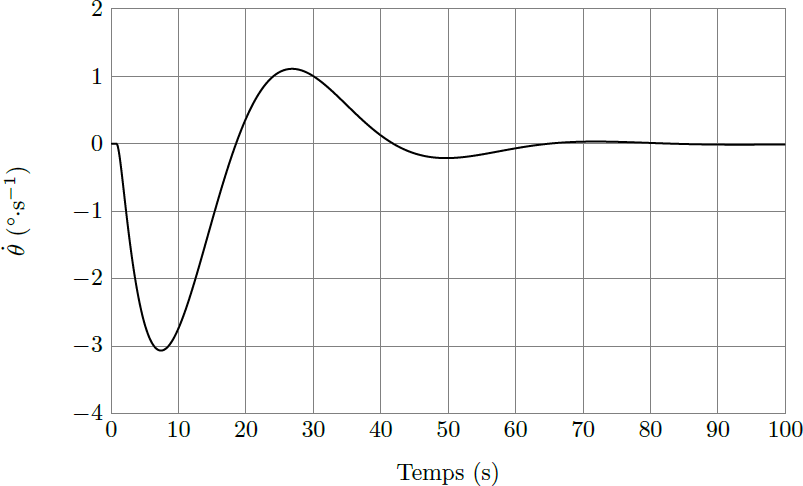
\includegraphics[width=.7\linewidth]{images/fig_13}
\caption{Évolution de la vitesse de rotation du satellite $\dot{\theta}$ (\si{\degres.s^{-1}}) en réponse à un dépointage initial de 20\degres \label{fig_13}}
\end{figure}
\fi


\question{\label{q_30}}\textit{La \autoref{fig_14} montre les réponses obtenues (en utilisant un simulateur trois axes comportant en particulier les modes oscillants dus aux souplesses de la structure) avec la loi de commande définie précédemment pour un dépointage initial $\Theta_0 = 20\degres$. Commenter les réponses obtenues et conclure alors sur la capacité de la nouvelle loi de commande à satisfaire l’ensemble des contraintes imposées par le cahier des charges.}
\ifprof
\begin{corrige}
D'après le cahier des charges : 
\begin{itemize}
\item couple maximal : $\SI{0,005}{Nm}$ : l'exigence est respectée, sauf ponctuellement au démarrage de la roue à réaction et au changement de loi de commande à $t=\SI{1300}{s}$;
\item vitesse maximale : $\SI{2800}{tr.min^{-1}} = \SI{293}{rad.s^{-1}}$ : l'exigence est respectée, car la vitesse reste inférieure à $\SI{35}{rad.s^{-1}}$.
\end{itemize}
Ces résultats permettent de valider la nouvelle loi de commande.
\end{corrige}
\else
\fi

\ifprof
\else

\begin{figure}[H]
\centering
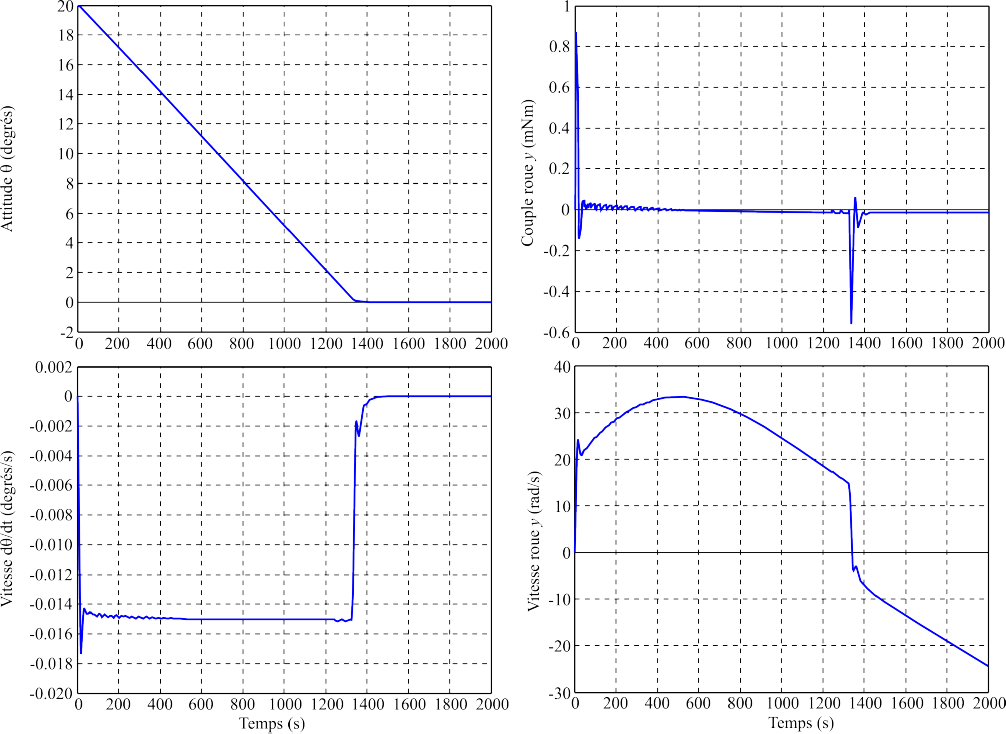
\includegraphics[width=.8\linewidth]{images/fig_14}
\caption{Évolutions temporelles à partir d’une condition initiale (dépointage) $\theta_0 = 20\degres$ \label{fig_14}}
\end{figure}
\fi

\subsubsection{\label{sec:3:D:3} Analyse des performances vis-à-vis d’un couple perturbateur constant}

L’objet de cette partie est d’analyser les performances de la loi de commande lorsque le satellite est soumis à
un couple extérieur constant, $C_{\text{ext}}= C_0 \gamma(t)$ d’amplitude $C_0 =\SI{e-6}{Nm}$.

\question{\label{q_31}}\textit{Sans calcul, mais en justifiant votre réponse, préciser l’écart en régime permanent en réponse à un couple
perturbateur constant.}
\ifprof
\begin{corrige}
$C(p)=K\dfrac{\left(1+\tau p\right)^2}{p}$. Le correcteur contient une action intégrale en amont de la perturbation. Pour une perturbation constante, l'écart en régime permanent est donc nul.
\end{corrige}
\else
\fi

\question{\label{q_32}}\textit{À partir du schéma de la \autoref{fig_11}, déterminer la valeur du couple appliqué $C_{\text{roue}}$ en régime permanent
en réponse au couple perturbateur $C_{\text{ext}}(t)$ supposé constant et en déduire la loi temporelle d’évolution de la
vitesse de la roue. Quelle est la conséquence sur le fonctionnement de l’actionneur du couple perturbateur ? Justifier le terme de «~saturation~» pour décrire ce phénomène. À partir de quel horizon temporel survient cette
situation ?}
\ifprof
\begin{corrige}
On a $C_{\text{ext}}(t) = C_0 =\SI{e-6}{Nm}$. En régime permanent, $C_{\text{roue}}$ doit être égal à $-C_0 =-\SI{e-6}{Nm}$.

Par application du théorème du moment dynamique appliqué à la roue à réaction : $C_{\text{ext}}(t) = I_{ry} \dot{\omega}_r(t)$. On a donc $\omega_r(t) = -\dfrac{C_0}{I_{ry}}t + \text{cte}$.

Pour maintenir le couple désiré, il faut dont que la vitesse tende vers l'infini. La vitesse saturera donc à partir d'un certain seuil (ici \SI{2800}{tr/min}). 

En prenant la constante nulle, on a  $|\omega_r(T)| = \dfrac{C_0}{I_{ry}}T$ soit $T = \dfrac{2800 \times 2\pi}{60} \times 10^{6} \times 4\times 10 ^{-4} $ $=\SI{117 286}{s} \simeq \SI{32,5}{h}$.


\end{corrige}
\else
\fi

\ifprof
\else


Pour remédier au problème de saturation, on utilise des bobines magnétiques, appelées magnétocoupleurs, qui
permettent de créer des moments adaptés grâce à l’action du champ magnétique terrestre. Le satellite est équipé
de trois magnétocoupleurs orientés respectivement selon les trois directions $\vect{x}$, $\vect{y}$ et $\vect{z}$ du satellite, et dont on peut
commander précisément les moments magnétiques respectifs $\vect{\mathcal{M}}_x=\mathcal{M}_x\vect{x}$, $\vect{\mathcal{M}}_y=\mathcal{M}_y\vect{y}$ et $\vect{\mathcal{M}}_z=\mathcal{M}_z\vect{z}$. Dans
le cas d’une orbite polaire, le champ magnétique terrestre a pour expression $\vect{B}=B_0 \cos\left(\omega_0 t\right) \vect{x} +2 B_0 \sin\left(\omega_0 t\right) \vect{z}.$ L’interaction entre les magnétocoupleurs et le champ magnétique terrestre se traduit par un moment (mécanique)
dont l’expression au centre d’inertie $G$ du satellite est :
$$
\vect{M}_G (\text{magnétique}) = 
B_0 \left( 
2\mathcal{M}_y \sin \left(\omega_0 t \right) \vect{x}
+ \left(
\mathcal{M}_z \cos \left(\omega_0 t \right) 
-2\mathcal{M}_x \sin\left(\omega_0 t \right) \right)\vect{y}
-\mathcal{M}_y \cos \left(\omega_0 t \right) \vect{z}
\right).
$$
\fi

\question{\label{q_33}}\textit{Expliquer comment les magnétocoupleurs peuvent permettre de résoudre le problème de saturation des
roues de réaction : on détaillera précisément quel est le rôle de chacun des trois magnétocoupleurs et à quels
instants de l’orbite du satellite leurs effets sont les plus sensibles.}
\ifprof
\begin{corrige}
Les magnétocoupleurs coupleurs permettent d'apporter un couple supplémentaire pour remédier au problème de saturation.... 
\end{corrige}
\else
\fi